\documentclass[twocolumn]{aastex62}
\emergencystretch=1.em

\usepackage{amsmath,amsthm,amsfonts,amssymb,bm}
% for big dot
\makeatletter
\newcommand*\bigcdot{\mathpalette\bigcdot@{.5}}
\newcommand*\bigcdot@[2]{\mathbin{\vcenter{\hbox{\scalebox{#2}{$\m@th#1\bullet$}}}}}
\newcommand{\argmax}{\mathop{\rm arg~max}\limits}
\newcommand{\argmin}{\mathop{\rm arg~min}\limits}

\usepackage{listings}
\usepackage{physics}
\usepackage{multirow}
\usepackage{color}
\usepackage{graphicx,subfigure}
\renewcommand\thesubfigure{(\roman{subfigure})}

\usepackage{textcomp}
\usepackage{epstopdf}
\usepackage{natbib}
\usepackage{commath}
\hypersetup{breaklinks}

\DeclareMathOperator{\arccosh}{arccosh}
\newcommand \redColor{\color{red}}

\renewcommand\labelenumi{(\roman{enumi})}
\renewcommand\theenumi\labelenumi

\usepackage{algorithm,algcompatible}
\usepackage[-]{callouts}

%\DeclareMathOperator*{\argmax}{\arg\!\max}
\algnewcommand\INPUT{\item[\textbf{Input:}]}
\algnewcommand\OUTPUT{\item[\textbf{Output:}]}

\newcommand{\includezraphics}[1]{
\begin{annotate}{
\includegraphics[width=0.43\textwidth]{#1}}{0.45}
\arrow { -6., -4}{ -6., 4}
\note {-6.,4.5}{$\huge{z}$}
\end{annotate}
}

\makeatother
%\newcommand{\jcap}{JCAP}

\begin{document}
\title{Sparsity Weak Lensing $3$-D Density Map Reconstruction:
Reducing the line of sight smearing}
%\author{Xiangchong Li}
%\affiliation{Department of Physics, University of Tokyo, Tokyo 113-0033, Japan}
%\affiliation{Kavli Institute for the Physics and Mathematics of the Universe (WPI),\\
%University of Tokyo, Kashiwa 277-8583, Japan}
%\author{Masamune Oguri}
%\affiliation{Department of Physics, University of Tokyo, Tokyo 113-0033, Japan}
%\affiliation{Kavli Institute for the Physics and Mathematics of the Universe (WPI),\\
%University of Tokyo, Kashiwa 277-8583, Japan}
%\affiliation{Research Center for the Early Universe, University of Tokyo, Tokyo 113-0033, Japan}
%\author{Wentao Luo}
%\affiliation{Kavli Institute for the Physics and Mathematics of the Universe (WPI),\\
%University of Tokyo, Kashiwa 277-8583, Japan}
%\author{HSC Collaboration}
%\noaffiliation
%\email{xiangchong.li@ipmu.jp}

\begin{abstract}
A new method is developed to reconstruct $3$-D density contrast maps from
photometric weak-lensing shear measurements. The $3$-D density contrast maps
are modeled as a summation of the NFW basis atoms, which have $2$-D multi-scale
NFW surface density profiles on the transverse plane and $1$-D Dirac delta
functions in the line of sight direction. With the prior assumption that the
density fields have a sparse spatial distribution, the density fields are
reconstructed using an oracle algorithm: adaptive lasso. Our method is tested
with realistic simulations using the HSC-like shape estimation error and
photo-$z$ uncertainty.  Our findings are summarized as follows: 1) The lasso
solution suffers from a smear of structure in the line of sight direction even
in the absence of shape noise. The adaptive lasso algorithm significantly
removes the line of sight smear of structure.  2) The algorithm is able to
detect halo with minimal mass limits of $10^{14.0} M_{\odot}/h$, $10^{14.7}
M_{\odot}/h$, $10^{15.0} M_{\odot}/h$ for the low ($z<0.3$), median ($0.3\leq
z< 0.6$) and high ($0.6\leq z< 0.85$) redshifts, respectively, with a false
detection of 0.022/deg$^2$.  3) The estimated redshift of the halos detected
from the reconstructed mass maps are lower than the true redshift by about
$0.03$ for halos at low redshifts ($z\leq 0.4$). The relative redshift bias is
below $0.5\%$ for halos at $0.4<z\leq 0.85$.
\end{abstract}

\section{Introduction}

\begin{figure*}[!t] 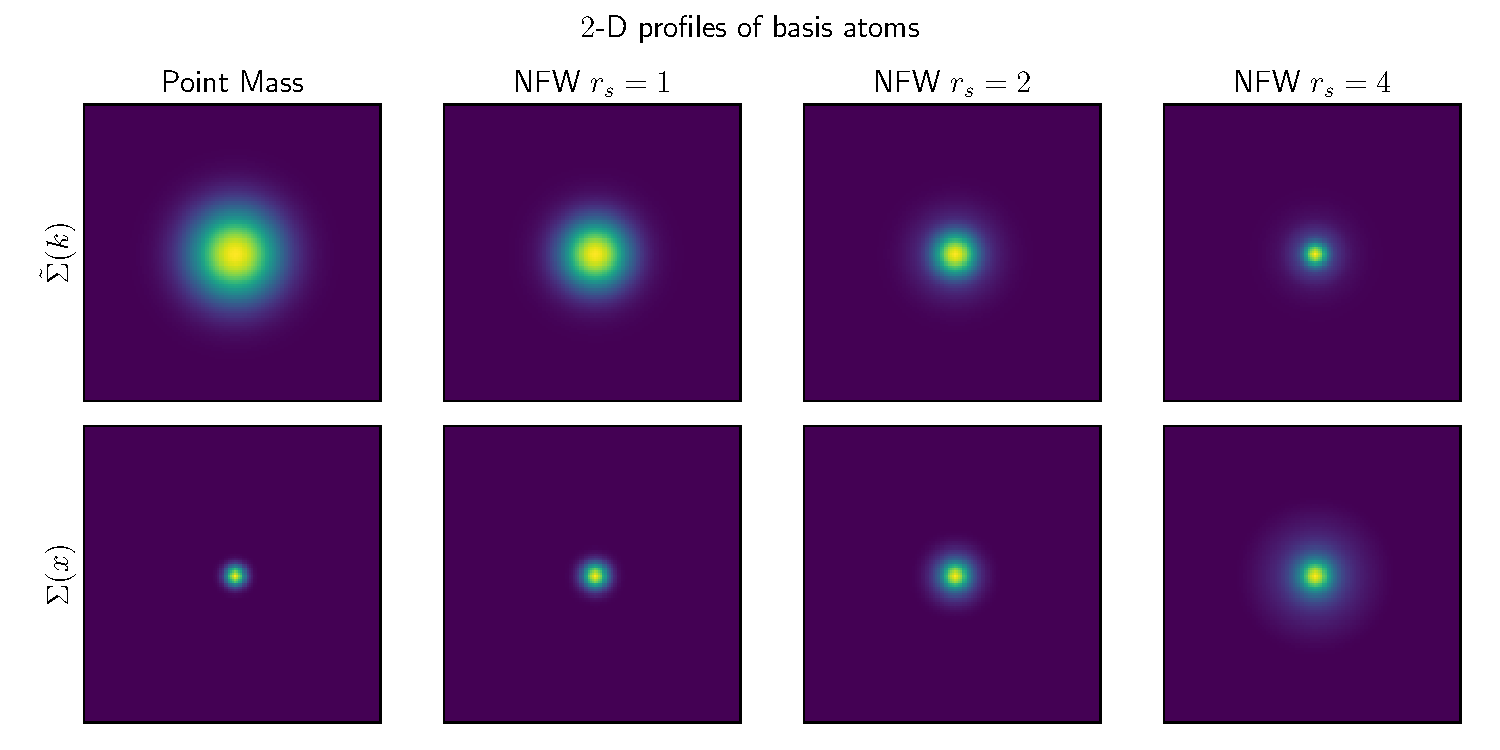
\includegraphics[width=1.\textwidth]{nfwlet-atom-2D.pdf}
    \caption{The smoothed pixelized basis atoms. The upper row shows the basis
        atoms in Fourier space, and the lower row shows the basis atoms in Real
        space.  The leftmost column is the point mass atom, and the other
        columns are the multi-scale NFW atoms.  The smoothing kernel is
        Gaussian with a standard dev
        iation of $1.5$ pixels.
        } \label{fig_atoms2D}
\end{figure*}

\begin{figure}
 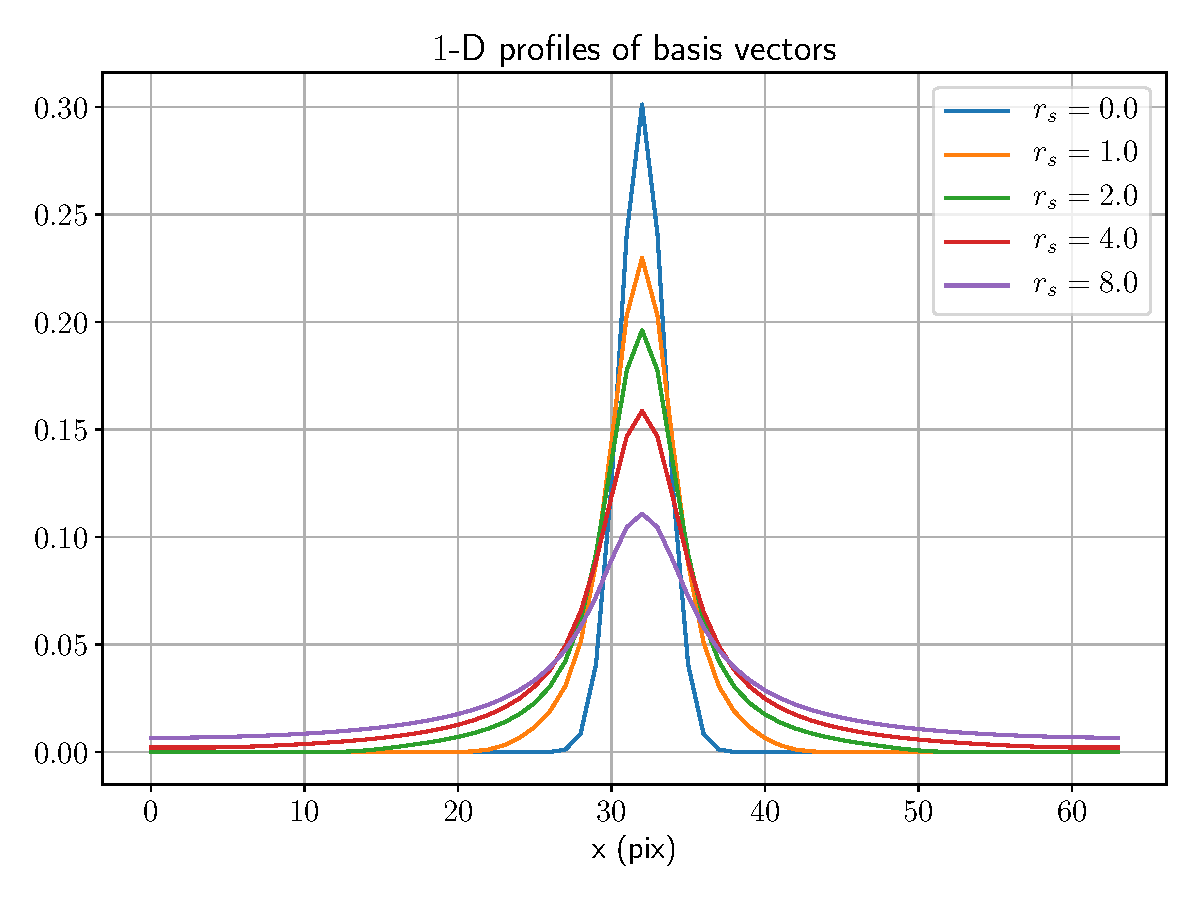
\includegraphics[width=0.5\textwidth]{nfwlet-atom-1D.pdf}
    \caption{The $1$-D slices for smoothed pixelized basis atoms at $x=0$. The
        corresponding $2$-D profiles are shown in Figure \ref{fig_atoms2D}.
        }
 \label{fig_atoms1D}
\end{figure}

Weak lensing refers to the phenomenon that light from distant galaxies is
distorted by the intervening inhomogeneous density distribution along the line
of sight due to gravity's influence.
As a result of the light distortion, the shapes of the background galaxies are
coherently distorted. The lensing effect imprints the information of
foreground mass density distribution to the background galaxy images and offers
a direct probe into the mass density distribution in our universe
\citep[see][for recent reviews]{revKilbinger15,revRachel17}.

The expected shear measurements ($\gamma$) on distant galaxies are related to
the foreground density contrast field ($\delta$) through a linear
transformation: \begin{equation} \label{eq-intro-delta2shear} \gamma=\mathbf{T}
\delta, \end{equation} where $\mathbf{T}$ is used to denote the linear
transformation operator, which includes not only physical lensing effect but
also systematic effects from observations (e.g., pixelization and smoothing of
the shear field in the transverse plane, photo-$z$ uncertainty).

Several large-scale surveys target to study the weak-lensing effect at a high
precision level (e.g., HSC \citep{HSC1-data}, KIDS \citep{KIDS13}, DES
\citep{DES05}, LSST \citep{LSSTScienceBook}, Euclid \citep{Euclid2011}, NGRST
\citep{WFIRST15}).

The primary goal of most weak-lensing surveys is to constrain the cosmology
model through $2$-point correlations. The studies include galaxy$-$galaxy
lensing, which cross-correlating the shear field ($\gamma$) with the positions
of foreground galaxies
\citep{gglens-GAMA-Han2014,gglens-BossCFHTMore2015,gglens-DES1}, and cosmic
shear which auto-correlates the shear measurements
\citep{cosmicShearRealKids450,cosmicShear-DES1,cosmicShear_HSC1_Chiaki2019,cosmicShear_HSC1_Hamana2019}.
Since the shear is directly related to the foreground matter distribution as
shown in eq.  (\ref{eq-intro-delta2shear}), Galaxy$-$galaxy lensing probes into
the correlation between the matter field and galaxy field. On the other hand,
cosmic shear probes into the auto-correlation of matter field.

The reconstruction of density map from shear measurements also receive
considerable interest as it reaches the nonlinear scales.  $2$-D density map
reconstruction which recover an integration of projected mass along the line of
sight has been well studied within the community
\citep{massMap-KS1993,WL-massMap-Glimpse2D-Lanusse2016,sparseBaysianMassMap-Price2020}
and applied to large-scale surveys
\citep{HSC1-massMaps,massMapDES-Chang2018,DES-SV-massMap-sparsity}. However,
the reconstruction of $3$-D mass map is still a challenging task.

To fully reconstruct the $3$-D mass density distribution ($\delta$) from the
photometric shear observations ($\gamma$), the density contrast field is
modeled as a summation of basis atoms in a model dictionary:
\begin{equation} \label{eq-intro-dict}
 \delta= \mathbf{\Phi} x,
\end{equation}
where $\mathbf{\Phi}$ is the transformation operator from the projection
coefficient field to the density contrast, and $x$ denotes the parameters.
\citet{LSS-massMap-Wiener-Simon2009} reconstruct the density field in Fourier
space, which is equivalent to model the mass field with sinusoidal functions.
On the other hand, \citet{LSS-massMap-Glimpse3D-Leonard2014} models the mass
field with Starlets \citep{Starlet-Starck2015}.

The projection coefficients are estimated by optimizing a regularized loss
function. The estimator is generally defined as
\begin{equation}
\hat{x}=\argmin_{x} \left\{ \frac{1}{2}\norm{\Sigma^{-\frac{1}{2}}(\gamma-
\mathbf{T\Phi} x)}_2^2+ \lambda C(x) \right\},
\end{equation}
where $\norm{\Sigma^{-\frac{1}{2}}(\gamma - \mathbf{T\Phi} x)}_2^2$ is the
$l^2$ chi-square term\footnote{weighted by the inverse of the diagonal
covariance matrix of the error on the shear measurements ($\Sigma$).} measuring
the residuals between the prediction and the data, while $C(x)$ is the
regularization term measuring the deviation of the estimation of the parameter
($x$) from the prior assumptions. The $l^p$ norm is defined as
\begin{equation}
\norm{x}_p=(\sum_{i} |x|^p_i)^{\frac{1}{p}}.
\end{equation}
Such estimation prefers the parameters that are able to describe the
observations and align with the prior assumptions.  The regularization
parameter $\lambda$ adjusts the relative weight between the observations and
prior assumptions in the optimization process.

\citet{LSS-massMap-Wiener-Simon2009} propose to use the Wiener filter, which is
also known as $l^2$ ridge regulation ($C=\norm{x}^2_2$), to find a regularized
solution in Fourier space. \citet{HSC1-massMaps} apply the method of
\citet{LSS-massMap-Wiener-Simon2009} to the first-year data of the Hyper
Suprime-Cam Survey \citep{HSC1-data}.  However, the density maps reconstructed
by this method suffer from smearing along the line of sight direction with a
standard deviation of $\sigma_z=0.2 \sim 0.3$.

\citet{LSS-massMap-Glimpse3D-Leonard2014} propose to use a derivative version
of $l^1$ lasso regulation ($C=\norm{x}^1_1$) to find a sparse solution in the
Starlets dictionary space \citep{Starlet-Starck2015}.
\citet{LSS-massMap-Glimpse3D-Leonard2014} apply a greedy coordinate descent
algorithm, which selects the steepest coordinate in each iteration, to find the
minimum of a non-convex loss function penalized with the firm thresholding
function. \citet{LSS-massMap-Glimpse3D-Leonard2014} significantly reduce the
smearing along the line of sight. However, the stability of the non-convex
optimization and greedy coordinate descent algorithm has not been fully
justified. Moreover, the Starlets functions are not designed to model the
profile of clumpy mass in the universe.

$N$-body simulations have shown that the dark matter is distributed in halos
connected by filaments, and the density profile of a single halo follows the
NFW function \citep{halo-NFW1997ApJ}.  We construct a model dictionary with the
multi-scale NFW atoms.  The atoms follow multi-scale surface density profiles
of the NFW functions \citep{haloModel-TJ2003-3pt} on the transverse plane.
Following \citet{LSS-massMap-Glimpse3D-Leonard2014}, we neglect the depth of
halos since the resolution scale of the reconstruction in the line of sight
direction is much larger than the halo scale. Therefore, we set the NFW atoms'
profile in the line of sight direction as the Dirac delta function.  Moreover,
we assume that the halos are sparsely distributed in the universe.  With the
sparsity prior, the adaptive lasso regularization \citep{AdaLASSO-Zou2006} is
used to reconstruct the density field.  We find that, in contrast to the lasso
estimator that smears the structure along the line of sight, the adaptive lasso
can significantly reduce the smearing effect.

Compared with \citet{LSS-massMap-Glimpse3D-Leonard2014}, our dictionary is
built up to describe the clumpy mass in the universe with a clear physical
motivation. Furthermore, the adaptive lasso algorithm is strictly convex and
can be directly optimized with the FISTA algorithm \citep{FISTA-Beck2009}
without relying on any greedy coordinate descent approaches. The stability of
this convex optimization has been well studied.

This paper is organized as follows.
In Section \ref{sec:Method}, we propose the new method for $3$-D density map
reconstruction.
In Section \ref{sec:Test}, we test the novel algorithm on HSC-like simulations.
In Section \ref{sec:Sum}, we summarize and discuss the future development of
the method.

\section{Methodology}
\label{sec:Method}

\begin{figure}[!t]
 \centering
 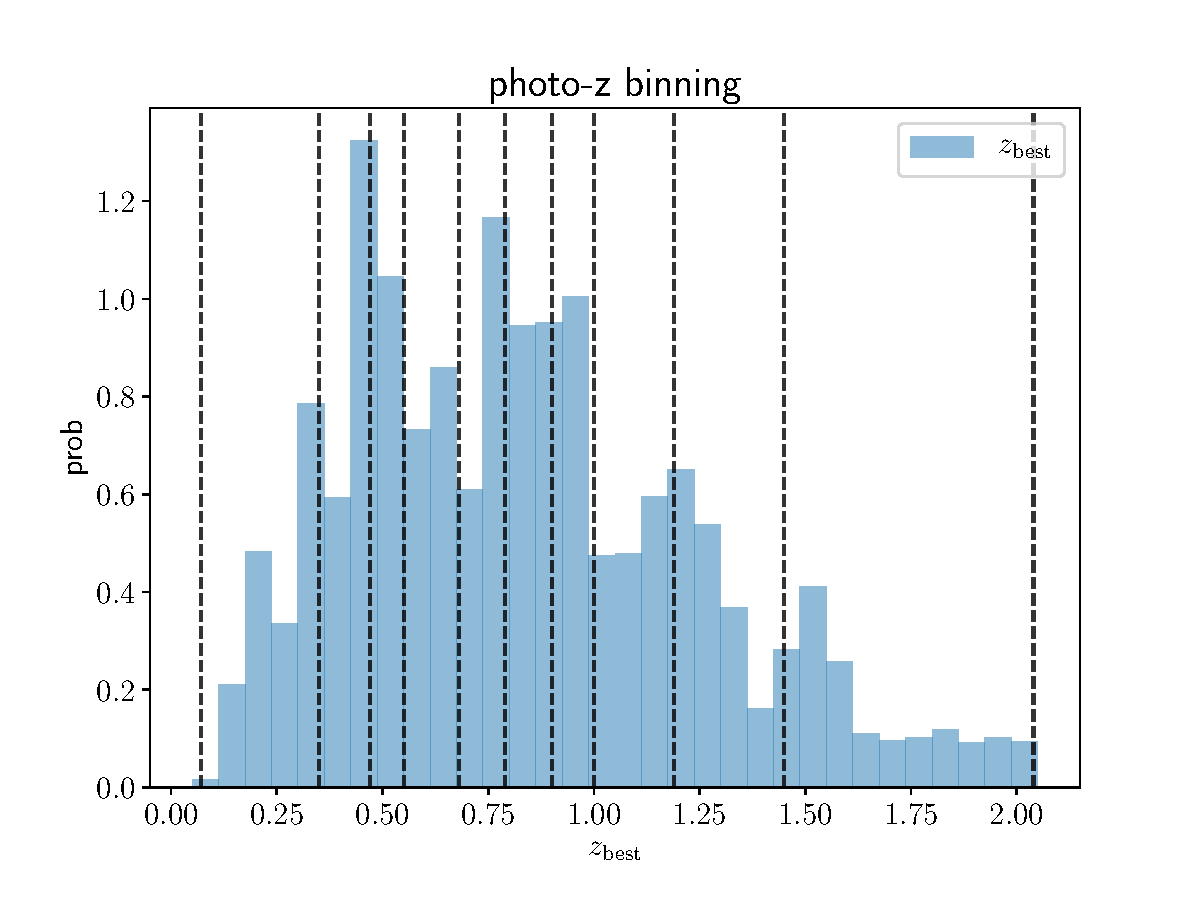
\includegraphics[width=0.5\textwidth]{photo-z_binning.pdf}
 \caption{The source galaxies are binned into $10$ redshift bins according to
     their Machine Learning and photo-Z (MLZ) best photo-$z$ estimation. The
     blue histogram is the normalized number distribution of the best photo-$z$
     estimation. The vertical dashed lines are the boundaries of the redshift
     bins.  The galaxies are equal-number binned.
        } \label{fig_bestpz}
\end{figure}

We first review the lensing process in section \ref{subsec:method-delta2shear}.
Then, we introduce the dictionary used to model the foreground density maps in
section \ref{subsec:method-dictionary}.

Subsequently, in section \ref{subsec:method-Systematics}, we discuss several
systematic effects from observations which include photo-$z$ uncertainty
(section \ref{subsec:method-photoz}), smoothing (section
\ref{subsec:method-smoothing}), masking(section \ref{subsec:method-msknoise}),
and pixelization (section \ref{subsec:method-pixel}).

Finally, we solve the mass reconstruction problem in section
\ref{subsec:method-reconstruction} using the adaptive lasso algorithm
\citep{AdaLASSO-Zou2006} optimized with the FISTA algorithm
\citep{FISTA-Beck2009}.


\subsection{Lensing}
\label{subsec:method-delta2shear}

\begin{figure}[!t]
 \centering
 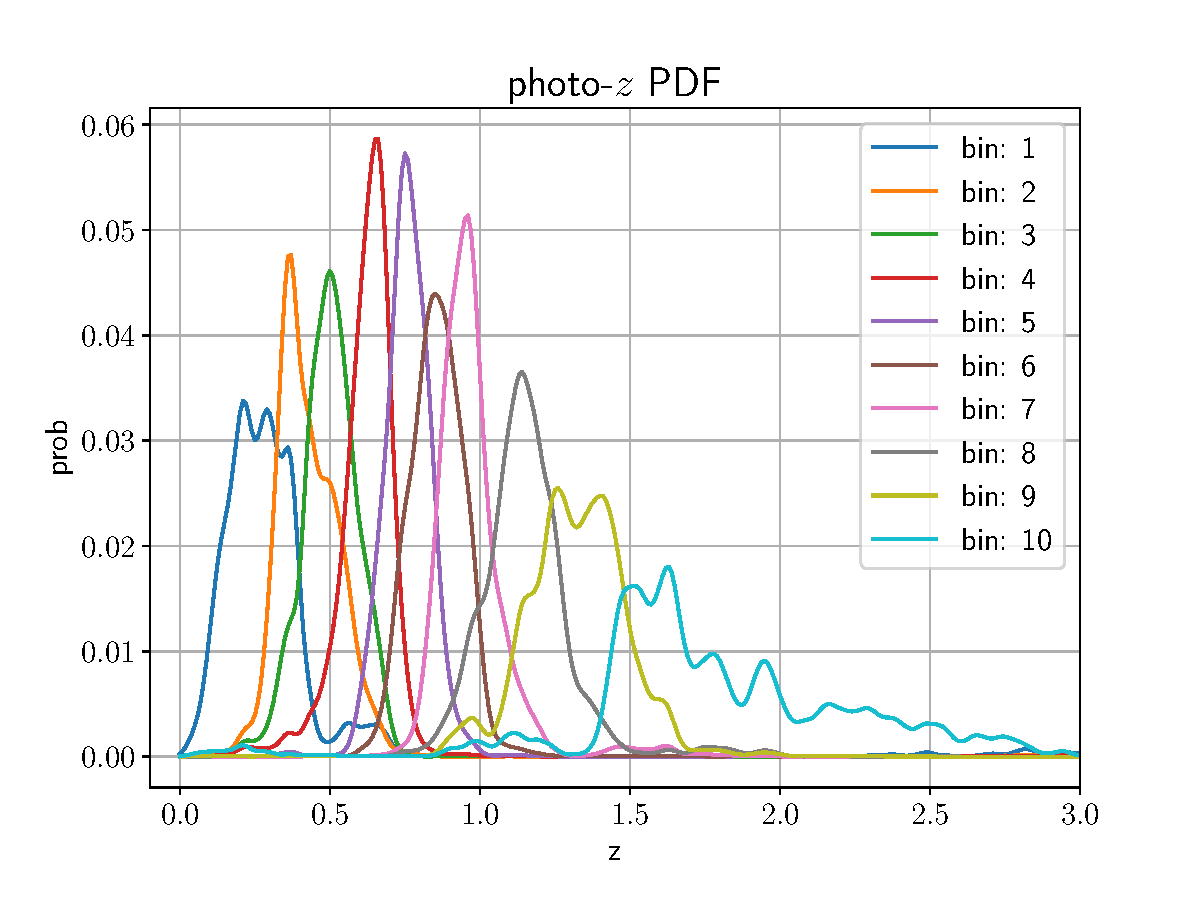
\includegraphics[width=0.5\textwidth]{mlz-poz.pdf}
 \caption{The average PDF of MLZ photo-$z$ error for $10$ source redshift bins.
        }\label{fig_pdfpz}
\end{figure}

The lensing convergence map at the comoving distance $\chi_s$ caused by the
foreground inhomogeneous density distribution at the comoving distance $\chi_l$
($\chi_l< \chi_s$) along the line of sight is
\begin{equation}
\kappa(\vec{\theta},\chi_s)=\frac{3H_0^2\Omega_M}{2 c^2} \int_0^{\chi_s} d\chi_l \frac{\chi_l \chi_{sl}}{\chi_s}
\frac{\delta(\vec{\theta},\chi_l)}{a(\chi_l)},
\end{equation}
where $\delta=\rho(\vec{\theta},\chi_l)/\bar{\rho}-1$ is the density contrast
at the position of lens, $H_0$ is the Hubble parameter, $\Omega_M$ is the
matter density parameter, $c$ is the speed of light, and $a(\chi_l)$ is the
scale parameter at the lens position.

After substituting comoving distance ($\chi$) with redshift ($z$), we have
\begin{equation}\label{eq-delta2kappa}
\kappa(\vec{\theta},z_s)=\int_0^{z_s} dz_l K(z_l,z_s)\delta(\vec{\theta},z_l).
\end{equation}
where $K(z_l,z_s)$ is the lensing kernel defined as
\begin{equation}
K(z_l,z_s) =
\begin{cases}
\frac{3H_0\Omega_M}{2 c} \frac{\chi_l \chi_{sl} (1+z_l)}{\chi_{s} E\left(z_l\right)} & (z_s>z_l),\\
0&(z_s \leq z_l),
\end{cases}
\end{equation}
where $E(z)$ is the Hubble parameter as a function of redshift, in units of $H_0$.

\begin{figure*}[!t]
 \centering
 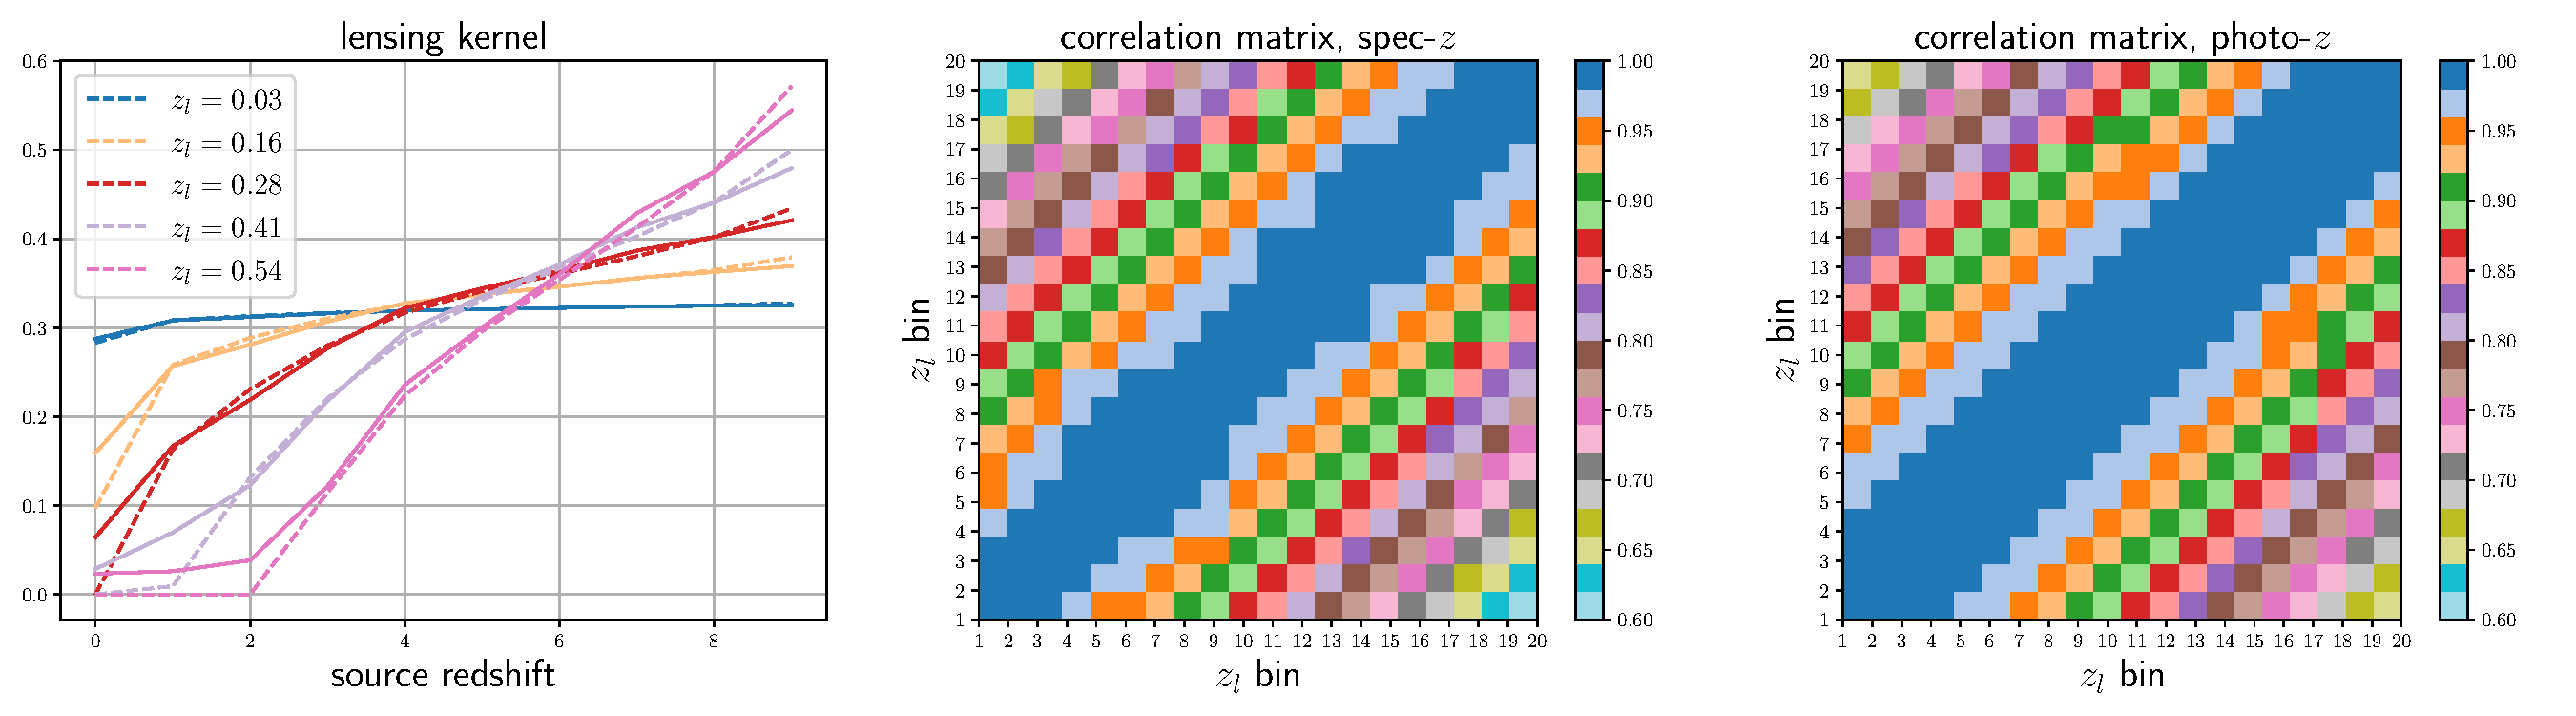
\includegraphics[width=1.\textwidth]{lensing_kernel.pdf}
 \caption{The left panel shows the lensing kernels for five different lens
         redshifts. The dashed lines are the kernels for spectroscopic redshift,
         which assumes that the source galaxies' redshifts are precisely
         estimated. The solid lines are for photometric redshifts, which
         accounts for the influence of photometric redshift uncertainty. The
         other two panels show the correlation between lensing kernels of
         different lens redshifts. The middle panel is for spectroscopic
         redshift, and the right panel is for photometric redshifts. The
         lensing kernels are normalized so that the diagonal elements of the
         correlation matrices equal one.
        }\label{fig_corlensKer}
\end{figure*}

As shown in \citet{massMap-KS1993}, the shear field is related to the kappa
field at the same redshift plane via
\begin{equation}\label{eq-kappa2gamma}
\gamma_L(\vec{\theta},z_s) = \int  d^2 \theta' D(\vec{\theta}-\vec{\theta'}) \kappa(\vec{\theta'},z_s),
\end{equation}
where
\begin{equation}
D(\vec{\theta})=-\frac{1}{\pi}(\theta_1-i\theta_2)^{-2}.
\end{equation}
Here we denote the physical shear distortion field as $\gamma_L$ and we note
that the final observed shear measurements are influenced by systematic errors
from observations. The systematic errors will be discussed in Section
\ref{subsec:method-Systematics}.

Combining equation (\ref{eq-delta2kappa}) with equation (\ref{eq-kappa2gamma}),
the expectation of lensing shear signal is
\begin{equation}\label{eq-delta2gammat}
\gamma_L(\vec{\theta},z_s) = \int_0^{z_s} dz_l K(z_l,z_s) \int d^2 \theta' \vec{D}(\vec{\theta}-\vec{\theta'}) \delta(\vec{\theta'},z_l).
\end{equation}

To simplify the expression, we define the lensing transform operator as
\begin{equation}
\mathbf{Q}=\int_0^{z_s} dz_l K(z_l,z_s) \int d^2 \theta'  \vec{D}(\vec{\theta}-\vec{\theta'}),
\end{equation}
and eq. (\ref{eq-delta2gammat}) is simplified to
\begin{equation} \label{eq-delta2gammat-simp}
\gamma_L=\mathbf{Q}\delta.
\end{equation}

\subsection{Dictionary}
\label{subsec:method-dictionary}

\begin{figure*}[!t]
\centering
\subfigure[lasso]{\includezraphics{delta-3-7-pz-nn-lasso.pdf}}
\subfigure[adaptive lasso]{\includezraphics{delta-3-7-pz-nn-alasso.pdf}}
\caption{The density map reconstructions with the lasso (left) and the adaptive
        lasso (right) algorithms. The input density map is from a NFW halo with
        mass $M_{200}=10^{15} ~h^{-1}M_{\odot}$ at redshift $0.35$. The lasso
        reconstruction smears the density field along the line of sight
        direction (vertical direction in the plots).  The vertical direction is
        the line of sight direction, and the lower boundaries and upper
        boundaries of the boxes are $z=0.01$ and $z=0.85$, respectively. Noises
        on galaxy shape measurements are neglected in this simulation.
        } \label{fig_lassoVsadaLasso}
\end{figure*}

The density contrast field is modeled as a summation of basis atoms in the
dictionary:
\begin{equation}\label{eq-x2delta}
\delta(\vec{r}) = \sum_{s=1}^{N} \int d^3 r' \phi_s(\vec{r}-\vec{r'}) x_s(\vec{r'}),
\end{equation}
where $\phi_s(\vec{r})$ are the basis atoms of the dictionary. The basis atoms
have `$N$' different scale frames, and the atoms in each scale frame are
shifted by $\vec{r'}$ to form models at different spatial positions.
$x_s(\vec{r'})$ is the projection coefficients of the density contrast field
onto the basis atoms.

We propose to use the multi-scale NFW atoms, denoted as
$\{\phi_1,...,\phi_N\}$, as the basis atoms of our dictionary.  On the
transverse plane, the NFW atoms follow surface density profiles of the NFW
halos \citep{haloModel-TJ2003-3pt} with scale radius $\theta_\alpha$ and
truncation radius $c \theta_\alpha$ , where $c$ is the concentration of the NFW
halos.  As the scales of halos are much smaller than the reachable redshift
resolution, we neglect the depth of halo on the line of sight direction and set
the NFW atoms' profiles in the line of sight direction to $1$-D Dirac delta
functions as suggested by \citep{LSS-massMap-Glimpse3D-Leonard2014}. The
multi-scale NFW atoms are defined as
\begin{equation}
\begin{split}
\phi_\alpha(\vec{r}) =&\frac{f }{2 \pi \theta_\alpha^2 }
F(|\vec{\theta}|/\theta_\alpha) \delta_D(z),\\
&  (s=1..N)
\end{split}
\end{equation}
where
\begin{equation}
F(x)=
\begin{cases}
-\frac{\sqrt{c^2-x^2}}{(1-x^2)(1+c)} + \frac{\arccosh
\left(\frac{x^2+c}{x(1+c)}\right)}{(1-x^2)^{3/2}}  & (x<1),\\
\frac{\sqrt{c^2-1}}{3(1+c)} (1+\frac{1}{c+1}) & (x=1),\\
-\frac{\sqrt{c^2-x^2}}{(1-x^2)(1+c)} +
\frac{\arccos\left(\frac{x^2+c}{x(1+c)}\right)}{(x^2-1)^{3/2}} & (1<x\leq c),\\
0& (x>c).
\end{cases}
\end{equation}
$f=1/[\ln (1+c)-c/(1+c)]$. In this work, we fix $c=4$ for the NFW atoms in
different scale frames.

To simplify the notation, we compress the projection coefficients into a column
vector:
$x=\begin{pmatrix}
x_{0}\\
x_{1}\\
...\\
x_{N}
\end{pmatrix}$,
and compress the dictionary transform operator to a row vector:
\begin{equation}
\mathbf{\Phi}=\begin{pmatrix}
\int d^3r\phi_0(\vec{r}) ~\int d^3r \phi_1(\vec{r})~ ...~\int d^3r \phi_{N}(\vec{r})
\end{pmatrix}.
\end{equation}
We substitute eq. (\ref{eq-x2delta}) into eq.(\ref{eq-delta2gammat}) and get
\begin{equation}\label{eq-x2gammat}
\gamma_L=\mathbf{Q}\mathbf{\Phi} x.
\end{equation}

In this paper, a dictionary constructed with point mass atoms is used to
compare with the dictionary of multi-scale atoms.  The point mass atoms is a
$3$-D Dirac function defined as follows
\begin{equation}
\phi_{\rm{PM}}(\vec{r})= \delta_D(\theta_1) \delta_D(\theta_2) \delta_D(z).
\end{equation}

The $2$-D profiles of the point mass atom and the multi-scale NFW atoms on the
transverse plane are shown in Figure \ref{fig_atoms2D}. The $1$-D slices of the
profiles are demonstrated in Figure \ref{fig_atoms1D}. Note that these profiles
are smoothed with a Gaussian kernel and pixelized into evenly spaced grids. The
smoothing operation is discussed in Section \ref{subsec:method-smoothing}, and
the pixelization operation is discussed in Section \ref{subsec:method-pixel}.

\subsection{Systematics}
\label{subsec:method-Systematics}

The observed shear measurements are deviated from the physical shear prediction
due to the systematic errors from observations. The influence of systematics is
carefully studied and incorporated into the forward modeling in this section.

\subsubsection{Photo-$z$ Uncertainty}
\label{subsec:method-photoz}

The photometric redshifts of source galaxies in the current large-scale survey
are estimated with a limited number of board photometric bands (e.g., $9$ bands
for KIDS$+$VIKING survey \citep{KIDS_VIKING-Hildebrant2020}, $5$ bands for DES
survey and HSC survey). As a result, the estimated redshifts of galaxies suffer
from much larger uncertainties than redshifts estimated with spectroscopic
observations. Such photo-$z$ uncertainty smears the lensing kernels
statistically since a galaxy with a best fit photo-$z$ estimation of $z_s$ has
possibilities of being actually located at different redshifts ($z$).  The
probability function for the photo-$z$ uncertainty is denoted as $P(z|z_s)$,
and the expected shear distortion on the galaxy is
\begin{equation}\label{eq-delta2gamma-poz}
\int dz_s P(z|z_s) \gamma_L(\vec{\theta},z_s).
\end{equation}
With the definition of photo-$z$ smearing operator:
\begin{equation}
\mathbf{P} = \int dz_s P(z|z_s),
\end{equation}
the photo-$z$ uncertainty changes the shear as
\begin{equation}
\gamma_L \rightarrow \mathbf{Q} \gamma_L,
\end{equation}
where we use $\rightarrow$ to denote the changes of shear by the systematic
operator.


Figure \ref{fig_bestpz} shows the histogram of the best Machine Learning and
photo-Z \citep[MLZ]{MLZ-TPZ2013} photometric redshift estimation from
\cite{HSC1-photoz} for galaxies in the tract 9347 of the HSC S16A data release
\citep{HSC1-data}. These Galaxies are divided into ten source galaxy bins
according to the photo-$z$ best estimation, and the boundaries of the bins are
shown as vertical dashed lines in Figure \ref{fig_bestpz}. Figure \ref{fig_pdfpz}
shows the average probability density function (PDF) for galaxies in each
redshift bin.

The left panel of Figure \ref{fig_corlensKer} shows the lensing kernels for
lenses at five different redshifts as functions of source galaxy redshift bins.
The dashed lines are the lensing kernel for spectroscopic redshifts with
neglectable redshift uncertainty. The solid lines are the lensing kernel for
photometric redshifts with redshift uncertainties shown in Figure
\ref{fig_pdfpz}.  As shown by the dashed lines in the left panel of Figure
\ref{fig_corlensKer}, the lensing kernels converge to zero for source redshifts
lower than the lens redshift if the uncertainties on the source galaxy
redshift estimations are neglectable. However, as demonstrated by the solid
lines in the same panel, for the source redshifts with large photo-$z$
uncertainties, the lensing kernels do not converge to zero at redshifts lower
than the lens redshift. This is because the galaxies with photo-$z$ estimations
lower than the lens redshifts may be actually located at higher redshifts due
to the photo-$z$ uncertainties.

The middle and right panels show the correlation between lensing kernels for
lenses at different redshifts. The middle panel is for spect-$z$, and the right
panel is for photo-$z$.  As demonstrated in the middle panel, the lensing
kernels are highly correlated even though the redshift estimation is precise.
Comparing the correlation matrices shown in the middle panel and the right
panel of Figure \ref{fig_corlensKer}, we conclude that the photo-$z$
uncertainties further increase the correlations between lensing kernels at
different lens plane.

\subsubsection{Smoothing}
\label{subsec:method-smoothing}

\begin{figure}[!t]
 \centering
 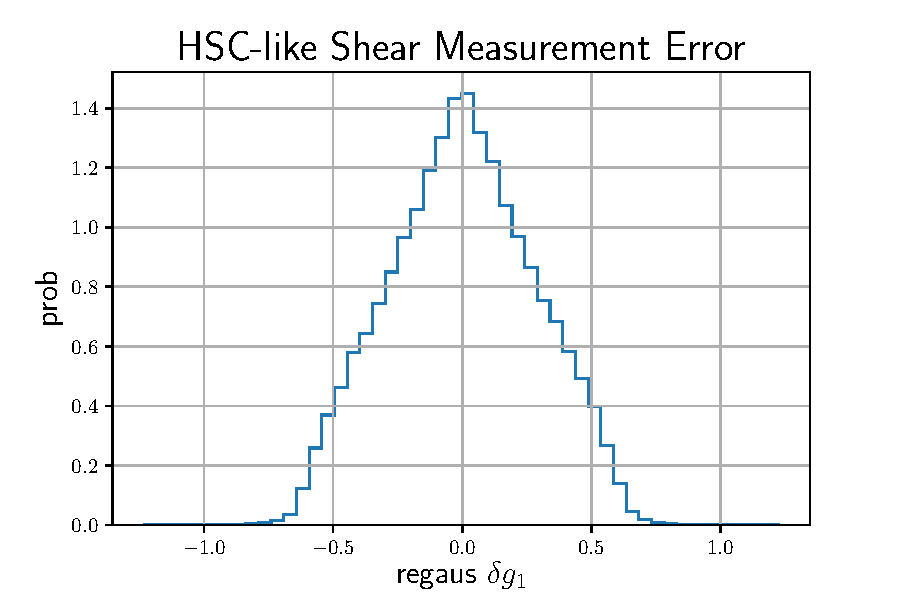
\includegraphics[width=0.5\textwidth]{shapeMeasurementError-HSCY1.pdf}
 \caption{The histograms of the HSC-like shape measurement error (including
         both from shape noise and from photon noise) on the first component of
         shear ($g_1$) for galaxies (blue lines) and smoothed pixels (orange
         lines). The solid steps are the sampled histograms, and the dashed
         lines are the normalized Gaussian distributions that have the same
         standard deviations as the corresponding histograms.
        }
 \label{fig_noiseHistogram}
\end{figure}

The observed galaxies have random irregular (unequally-spaced) spatial
distribution. To boost the computational speed, we smooth the shear
measurements from galaxy shapes and pixelize the smoothed measurements onto
regular grids.  After the pixelization, the fast Fourier transform (FFT) can be
directly conducted on the transverse plane in each source redshift bin.

The smoothing is conducted by convolving the shear measurements with a
smoothing kernel:
\begin{equation}
\gamma_{\rm{sm}} (\vec{\theta})  = \frac{\sum_i
W(\vec{\theta}-\vec{{\theta}}_i,z-z_i) \gamma_i}{\sum_i
W(\vec{\theta}-\vec{{\theta}}_i,z-z_i) },
\end{equation}
where $W(\vec{\theta},z)$ is a $3$-D smoothing kernel. $\gamma_i$, $z_i$ and
$\theta_i$ are the shear, photometric reshift, and transverse position of the
`$i$-th' galaxy in the catalog.

$W(\vec{\theta},z)$ can be decomposed into a transverse component
$W_T(\vec{\theta})$ and a line of sight component
$W_\times(z)$ as
\begin{equation}
W(\vec{\theta},z)=W_T(\vec{\theta}) W_\times (z).
\end{equation}
In this paper, we use an isotropic $2$-D Gaussian kernel and a $1$-D top-hat
kernel to smooth the measurements in the transverse plane and the line of sight
direction. These components of the smoothing kernel are
\begin{equation}
\begin{split}
W_T(\vec{\theta}) &=\frac{1}{2\pi\beta^2}\exp(-\frac{|\vec{\theta}|}{2\beta^2}),\\
W_\times (z) &=
\begin{cases}
1/\Delta z& (|z|<\Delta z/2),\\
0& else.
\end{cases}
\end{split}
\end{equation}
In this paper, we set $\beta=1.\arcmin5$.

Since the smoothing kernel is normalized by definition:
\begin{equation}
\int d^3r W(\vec{r})=1,
\end{equation}
with the approximation that the density of galaxy number - $n(\vec{r})$ -
varies slowly at the smoothing scale, the
smoothed galaxy number density:
\begin{equation}\label{eq-numDesSmooth}
n_{\rm{sm}}(\vec{r})=\sum_i W(\vec{\theta}-\vec{\theta_i},z-z_i),
\end{equation}
equals the galaxy number density: $n_{\rm{sm}}(\vec{r})=n(\vec{r})$.
We note that the galaxy number density experience a steep drop on the boundary
of the survey, therefore the smoothed galaxy number density does not equal the
galaxy number density close to the boundary of the survey.

The smoothing operator is defined as
\begin{equation}
\mathbf{W} = \int d^3 r' W(\vec{r}-\vec{r'}),
\end{equation}
and the smoothing procedure influence the shear signal through
\begin{equation}
\gamma_L \rightarrow \mathbf{W} \gamma_L.
\end{equation}

As we will discuss in Section \ref{subsec:method-pixel}, the smoothed shear
field is pixelized into equally spaced grids. We note that another widely used
scheme is to average the shear measurements in each pixel.  Such a scenario is
equivalent to resampling the shear field smoothed with a $3$-D top-hat kernel
with the same scale as the pixels.

\begin{figure}[!t]
 \centering
 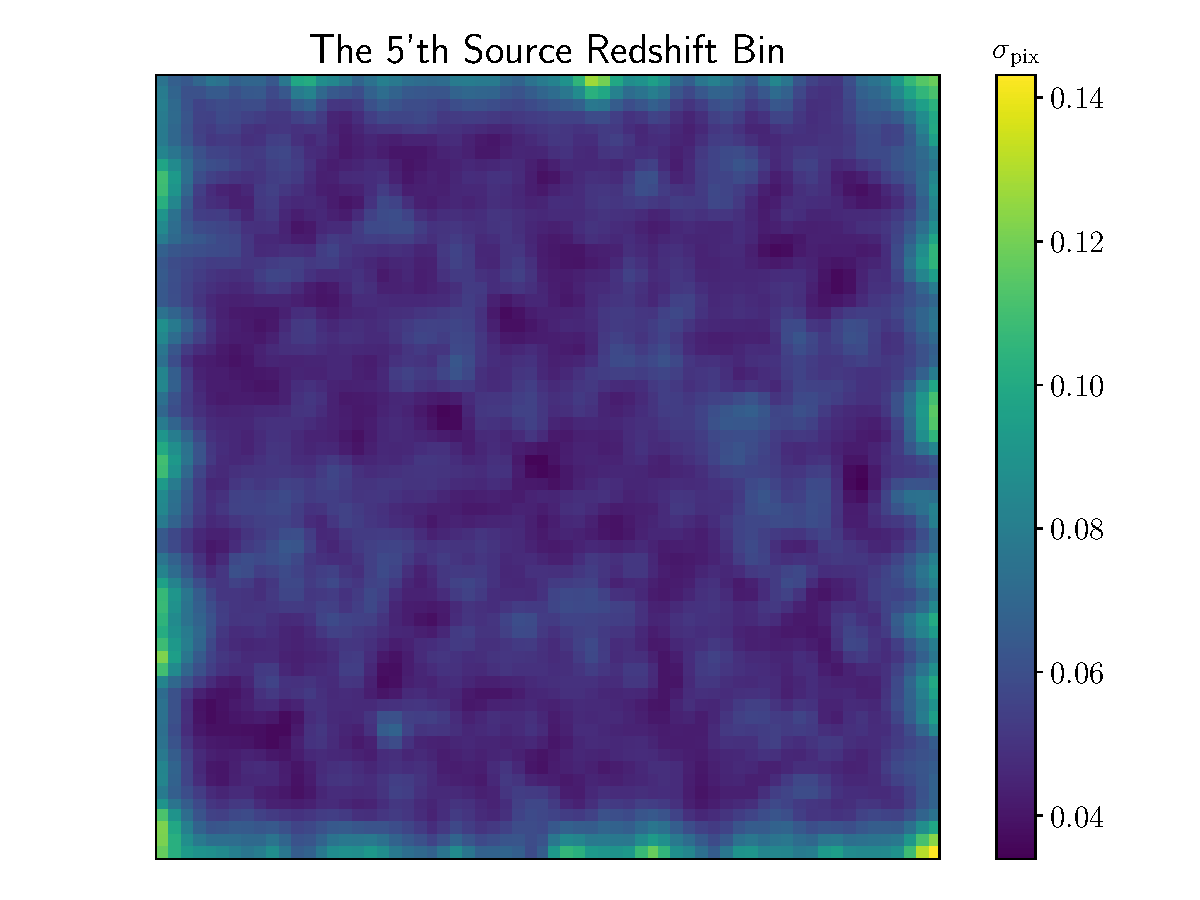
\includegraphics[width=0.5\textwidth]{noise_std_map_pix.pdf}
 \caption{The standard deviation pixel map of the HSC-like shape measurement error for the fifth source galaxy bin
        ($0.69 \leq z < 0.80 $).
        } \label{fig_noistdmap}
\end{figure}

\subsubsection{Masking}
\label{subsec:method-msknoise}

\begin{figure*}[!t]
 \centering
 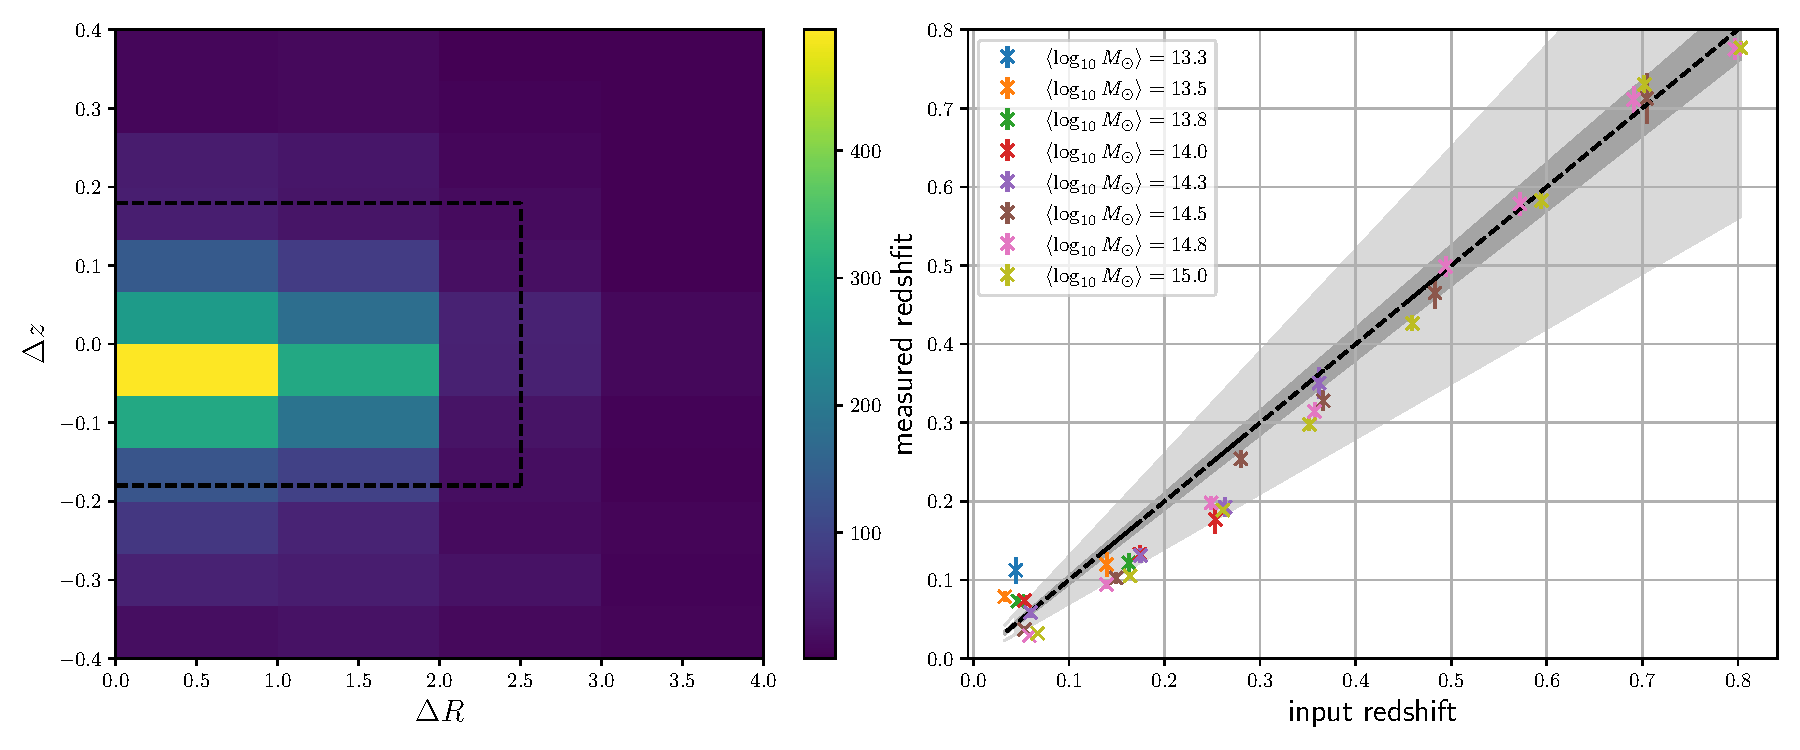
\includegraphics[width=1.0\textwidth]{peak_scatters_f3-1.pdf}
 \caption{The left panel shows the stacked $2$-D distribution of the deviations
     of detected peak positions from the centers of the corresponding input
     halos. The $x$-axis is for the deviated distance in the transverse plane,
     and the $y$-axis is for the deviation of the redshift. For each
     simulation, the positive peak inside the dashed black box with the
     minimal offset (in the pixel unit) from the input halo's position is
     taken as a true detection. The right panel focuses on the deviation of
     detected peaks in the line of sight direction. The $x$-axis is the input
     halo redshifts, and the $y$-axis is the redshift of the detected peak. The
     `$\cross$' denotes the average redshift of detected peaks for each halo
     over different noise realizations, and the error-bars are the
     uncertainties of the average redshifts. The deep gray area is for the
     relative redshift bias less than $0.05$, and the light gray area is for
     the relative redshift bias less than $0.5$. These results in this figure
     are based on the NFW dictionary with $\lambda=3.5$.
     } \label{fig_detoffsets}
\end{figure*}

In real observations, shear measurements are available in a finite region of
the sky, and the boundary of the region is always irregular. Moreover, many
isolated sub-regions near the bright stars are masked out since the light from
bright stars tends to influence the shear measurements on neighboring galaxies.

We define the masking window function according to the smoothed number density
(defined in eq. (\ref{eq-numDesSmooth})) of the galaxies:
\begin{equation}
 M(\vec{r})=
\begin{cases}
0 & n_{\rm{sm}}>1,\\
1 & \rm{else}.
\end{cases}
\end{equation}
The mask changes the shear measurements though
\begin{equation}\label{eq-delta2gamma-final}
\gamma_L(\vec{\theta},z) \rightarrow M(\vec{\theta},z) \gamma_L(\vec{\theta},z),
\end{equation}
We define the masking operator as
\begin{equation}
\mathbf{M}= \int d^3 r' M(\vec{r'}) \delta_D(\vec{r}-\vec{r'}),
\end{equation}
where $\delta_D(\vec{r})$ is $3$-D Dirac delta function. The shear is
influenced by the masking by
$\gamma_L \rightarrow \mathbf{M} \gamma_L$.

The final observed shear field, taking into account all of the systematics as
mentioned above from observations, is
\begin{equation}\label{eq-x2gamma-final}
\gamma =\mathbf{M} \mathbf{W} \mathbf{P} \mathbf{Q} \mathbf{\Phi} x.
\end{equation}
For simplicity, we denote $\mathbf{A}=\mathbf{M} \mathbf{W} \mathbf{P}
\mathbf{Q} \mathbf{\Phi} $ and
eq. (\ref{eq-x2gamma-final}) is written as
\begin{equation}\label{eq-x2gamma-simple}
\gamma=\mathbf{A} x.
\end{equation}

\subsubsection{Pixelization}
\label{subsec:method-pixel}

\begin{figure*}[!t]
 \centering
 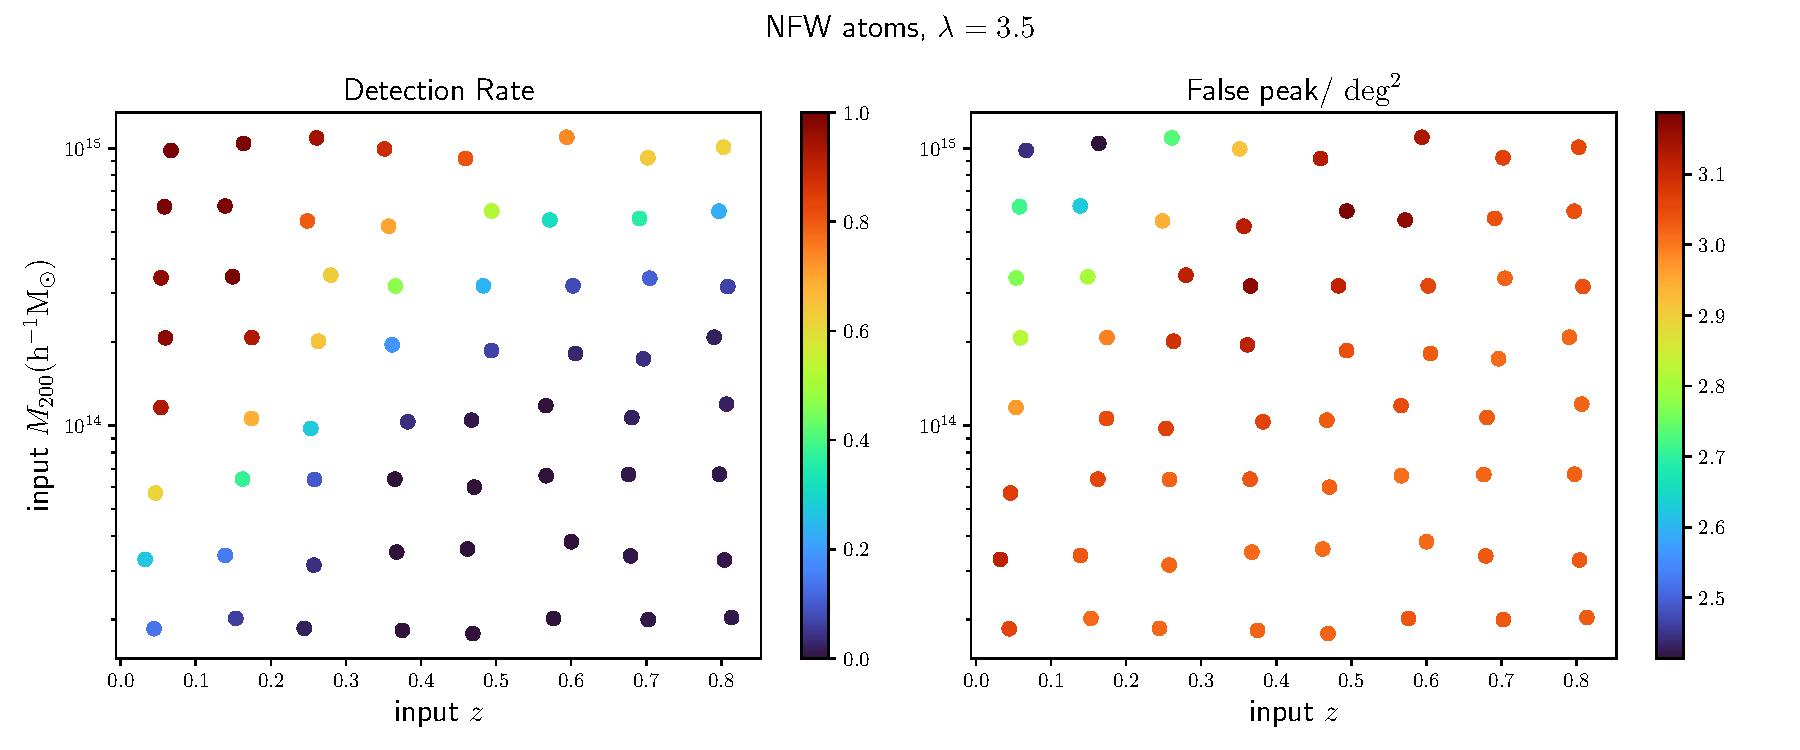
\includegraphics[width=1.0\textwidth]{detfalseRate_f3-1.pdf}
 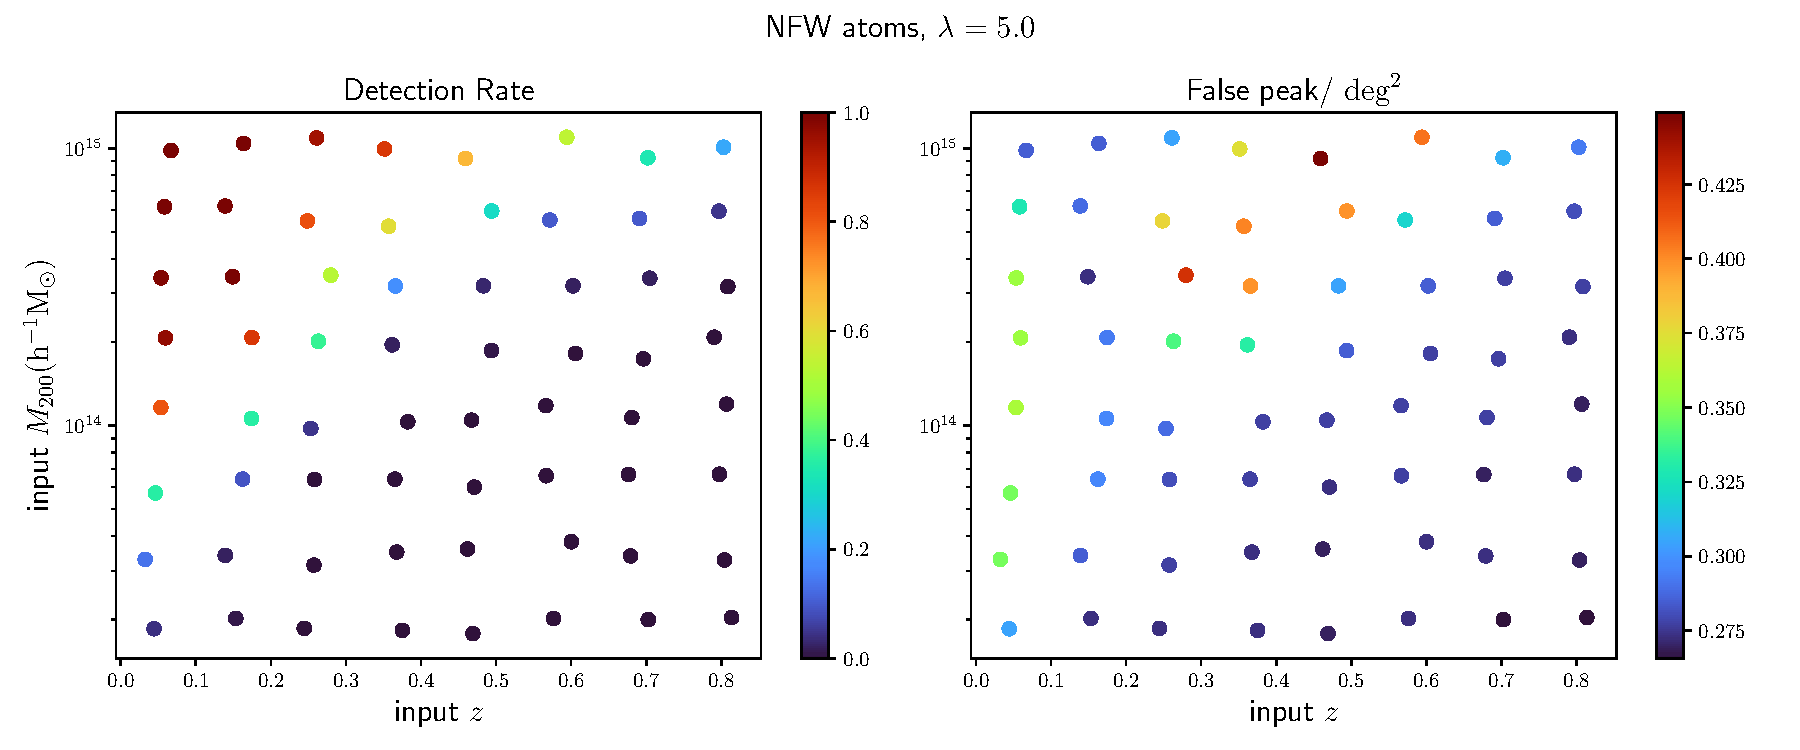
\includegraphics[width=1.0\textwidth]{detfalseRate_f3-3.pdf}
 \caption{The upper panels show the halo detection rate and the number of false
     peaks per square degree for mass map reconstructed with the NFW atoms. The
     penalization parameter is set to $\lambda=3.5$ for the upper panels.  The
     low panels show the results for $\lambda=5.0$.
        } \label{fig_detFalsRateNFW}
\end{figure*}

We pixelize the smoothed shear field into an $N_\theta \times N_\theta \times
N_s$ grid, where $N_\theta$ is the number of pixels for the two orthogonal axes
of the transverse plane and $N_s$ is the number of pixels for the line of sight
axis. $\gamma_{\alpha}$ denotes the smoothed shear measurements recorded on the
pixel with index $\alpha$, where $\alpha=1...N_\theta \times N_\theta \times
N_s$. The grids on the transverse planes are equally spaced with a pixel size of
$1\arcmin$.  Fast Fourier transform (FFT) can be used to boost the speed of
linear operation on the transverse plane, whereas the grids in the line of sight
direction follow equal number binning as shown in Figure \ref{fig_bestpz}.

Similarly, we pixelize each scale frame of the projection coefficient field $x$
into an $N_\theta \times N_\theta \times N_l$ grid. The pixelization on the
transverse plane for each scale frame is the same as that of the
smoothed shear field on the transverse plane. At the same time, the projection
coefficient field is pixelized into equal spaced grids in the line of sight
direction ranging from redshift $0.01$ to redshift $0.85$. Here, we use $N_l$
to denote the number of the lens planes and $x_{\beta}$ to denote the
projection parameter indexed as $\beta$, where $\beta=1...N_\theta \times
N_\theta \times N_l \times N$. The corresponding pixelized elements of the
forward transform matrix $\mathbf{A}$ is denoted as $A_{\alpha\beta}$.

We term the column vectors of the forward transform matrix $\mathbf{A}$ as the
effective basis atoms. We note that the effective basis atoms have different
$l^2$ norm. The $l^2$ norm of the $i'th$ column vectors of the effective basis
atoms are $\mathcal{N}_{i}=\sum_\alpha A_{i\alpha}A_{i\alpha}$. Before solving
the density map reconstruction problem, we normalize the column vectors of the
transform matrix through a rescaling:
\begin{equation}
\begin{split}
A'_{\alpha\beta}&=A_{\alpha\beta}/\mathcal{N}_{\alpha}^{\frac{1}{2}},\\
x'_{\beta}&=x_{\beta}\mathcal{N}_{\beta}^{\frac{1}{2}}.\\
\end{split}
\end{equation}

\subsection{Density map reconstruction}
\label{subsec:method-reconstruction}

\subsubsection{Adaptive lasso}

The lasso algorithm uses $l^1$ norm of the projection coefficient field to
regularize the modeling, and the estimator is defined as
\begin{equation}
\hat{x'}^{\rm{lasso}}=\argmin_{x} \left\{ \frac{1}{2}\norm{\Sigma^{-\frac{1}{2}}(\gamma- \mathbf{A'} x')}_2^2+ \lambda_{\rm{ls}} \norm{x'}^1_1\right\},
\end{equation}
where $\norm{\bigcdot}_1$ and $\norm{\bigcdot}_2$ refer to the $l^1$ norm and
$l^2$ norm, respectively.  $\lambda_{ls}$ denotes the penalization parameter
for the lasso estimation.

The lasso algorithm selects the parameters relevant to the measurements and
simultaneously estimates the value of the selected parameters.  However, it has
been shown by \citet{AdaLASSO-Zou2006} that when the column vectors of the
transforming matrix $\mathbf{A'}$ are highly correlated, the lasso cannot
select the relevant parameters from the parameter space consistently.
Moreover, the estimated parameters are biased due to the shrinkage in the lasso
regression. We note that, for the density map reconstruction problem, the
column vectors are highly correlated even in the absence of photometric
redshift uncertainties because, as shown in Figure \ref{fig_corlensKer}, the
lensing kernels for lenses at different redshifts are highly correlated.
Therefore, the lasso algorithm cannot select the consistent mass in the line of
sight direction, and the reconstructed mass suffers from smears in the line of
sight direction even in the absence of noise on shear measurements.  Figure
\ref{fig_lassoVsadaLasso} shows the reconstructions of a single halo's mass map
with halo mass equals $M_{200}=10^{15} ~h^{-1}M_{\odot}$ at redshift $0.35$.
The noises on shear measurements are not included in the simulation.  The left
panel of Figure \ref{fig_lassoVsadaLasso} is the reconstruction with the lasso
algorithm, which shows a significant smear along the line of sight.

\citet{AdaLASSO-Zou2006} proposes the adaptive lasso algorithm, which uses
adaptive weights to penalize different projection coefficients in the $l^1$
penalty. The adaptive lasso algorithm is a two-steps process. In the first
step, the lasso is used to estimate the parameters, and the preliminary
estimation of the lasso is denoted as $\hat{x'}^{\rm{lasso}}$. In the second
step, the preliminary lasso estimation is used to weight the penalization. The
weight on penalty is defined as
\begin{equation}
\hat{w}= \frac{1}{\abs{\hat{x'}^{\rm{lasso}}}^\tau},
\end{equation}
where we set the hyper-parameter $\tau$ to $2$.  The adaptive lasso estimator is
expressed as
\begin{equation}\label{eq-lossFun}
\hat{x'}=\argmin_{x'} \left\{ \frac{1}{2} \norm{\Sigma^{-\frac{1}{2}}(\gamma-\mathbf{A'}x')}^2_2 +
\hat{w}\lambda_{\rm{als}} \norm{x'}^1_1\right\}.
\end{equation}
Here, $\lambda_{\rm{als}}$ is the penalization parameter for the adaptive
lasso.  We note that $\lambda_{\rm{als}}$ does not need to be the same as the
penalization parameter for the preliminary lasso estimation
($\lambda_{\rm{ls}}$).

We rewrite the loss function with the Einstein notation:
\begin{equation}
\begin{split}
L(x')&=\frac{1}{2}(\Sigma^{-1})_{\alpha\beta}(\gamma^{*}_{\alpha}-A'^{*}_{\alpha i}x'_{i})
(\gamma_{\beta}-A'_{\beta j}x'_{j})\\
&+ \lambda_{\rm{als}} \hat{w_\beta} \abs{x'_\beta}.
\end{split}
\end{equation}
To simplify the notification in future, we define the quadruple term in the
loss function as $G(x')$:
\begin{equation}
G(x')=\frac{1}{2}\Sigma^{-1}_{\alpha\beta}(\gamma^{*}_{\alpha}-A'^{*}_{\alpha
i}x'_{i}) (\gamma_{\beta}-A'_{\beta j}x'_{j}).
\end{equation}


\subsubsection{FISTA}

\begin{figure}[!t]
 \centering
 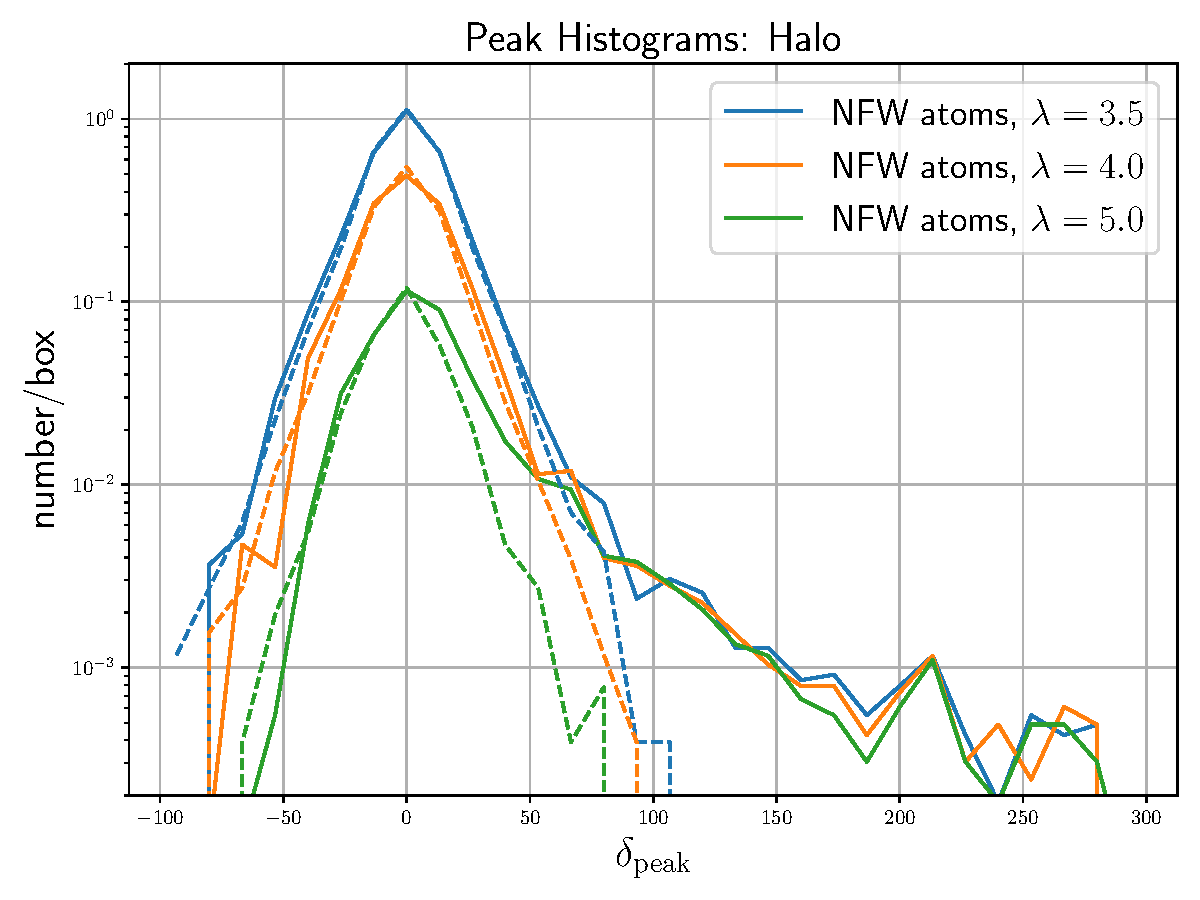
\includegraphics[width=0.5\textwidth]{peak_histograms.pdf}
 \caption{The histograms of detected peak values from all of the simulations.
     The solid lines with different colors are the results of reconstructions
     with the NFW dictionary penalized with different regularization
     parameters: $\lambda=3.5,4.0,5.0$. The dashed lines are the corresponding
     results of reconstructions from pure noise fields.
    }\label{fig_peakHist}
\end{figure}

\citet{FISTA-Beck2009} propose the Fast Iterative Soft Thresholding Algorithm
(FISTA) to solve the lasso problem.  Since the lasso's loss function and the
adaptive lasso's loss function only differ in their penalization terms. The
FISTA is also applicable to the adaptive lasso problem. We apply the FISTA to
solve both the preliminary lasso estimation and the final adaptive lasso
estimation.

Here we start from the lasso preliminary estimation. The coefficients are
initialized as $x_i^{(1)}=0$. According to the FISTA algorithm, we iteratively
update the projection coefficient field ($x$). Taking the $n$'th iteration as
an example, a temporary update is first calculated as
\begin{equation}
x'^{(n+1)}_{i}=\mathrm{ST}_{\lambda} \left(x'^{(n)}_{i} -\mu \partial_i G(x'^{(n)})\right),
\end{equation}
where $\mathrm{ST}$ is the soft thresholding function defined as
\begin{equation}
\mathrm{ST}_{\lambda} \left(x'\right) = \mathrm{sign} (x') \max \left(\abs{x'}-\lambda,0\right).
\end{equation}
The soft thresholding is a part of the lasso algorithm. It selects the
estimations with amplitude larger than $\lambda$, and shrink the estimations by
$\lambda$.
$\mu$ is the step size of the gradient descent iteration.  $\partial_i
G(x'^{(n)})$ refers to the $i$'th element of the gradient vector of $G$ at
point $x'^{(n)}$:
\begin{equation}
\partial_i G(x'^{(n)})=\Sigma^{-1}_{\alpha\beta}\Re\left(A'^{*}_{\alpha i}(\gamma_{\beta}-A'_{\beta j}x'_{j})\right),
\end{equation}
where $\Re\left( \bullet \right)$ is the function returns the real part of the
input function. The FISTA algorithm requires an additional update amounting to a
weighted average between
$x'^{(n+1)}$ and $x'^{(n)}$:
\begin{equation}
\begin{split}
t^{(n+1)}&=\frac{1+\sqrt{1+4(t^{(n)})^2}}{2},\\
x'^{(n+1)} &\leftarrow x'^{(x+1)}+ \frac{t^{(n)}-1}{t^{(n+1)}}(x'^{(n+1)}-x'^{(n)}),
\end{split}
\end{equation}
where the relative weight is initialized as $t^{(1)}=1$.

The FISTA algorithm converges as long as the gradient descent step size $\mu$
satisfies
\begin{equation}
 0< \mu < \frac{1}{ \norm{\mathbf{A^{\dagger}} \mathbf{\Sigma}^{-1} \mathbf{A} }},
\end{equation}
where $\norm{\mathbf{A^{\dagger}} \mathbf{\Sigma}^{-1} \mathbf{A} }$ refers to
the spectrum norm of the matrix $\mathbf{A^{\dagger}} \mathbf{\Sigma}^{-1}
\mathbf{A}$. The spectral norm is estimated by simulating a large number of
random vectors with $l^2$ norms equal one with different realizations. The
matrix operator $\mathbf{A^{\dagger}} \mathbf{\Sigma}^{-1} \mathbf{A}$ is
subsequently applied to each random vector and get a corresponding transformed
vector. The spectral norm of the matrix $\mathbf{A^{\dagger}}
\mathbf{\Sigma}^{-1} \mathbf{A}$ is determined as the maximum $l^2$ norm of the
transformed vectors.

As summarized in Algorithm \ref{alg-1}, we first initial the projection
coefficients as zero and use the FISTA algorithm to find the global minimum of
the lasso loss function. Such a global minimum is the preliminary estimation.
We then use the preliminary lasso estimation to weight the coefficients and
construct the adaptive lasso loss function. Finally, we set the preliminary
lasso estimation as the warm start of the adaptive lasso estimation and use the
FISTA algorithm again to find the adaptive lasso loss function's global minimum,
which is the final solution.


\begin{algorithm}[H]
\renewcommand{\thealgorithm}{}
\label{alg-1}
\caption{Our Algorithm}
\begin{algorithmic}[1]
\INPUT $\gamma$: Pixelized complex $3$-D array of shear
\OUTPUT  $\delta$: $3$-D array of density contrast
\STATE Normalize column vectors of $\mathbf{A}$
\STATE Estimate step size $\mu$ and $\mathbf{\Sigma}$
\STATE \textbf{Initialization:}
\STATE $x'^{(1)} = 0$
\STATE $\hat{w}=1$, $\lambda=\lambda_{\rm{ls}}$
\STATE $t^{(1)}=1$,$i=1$, $j=1$
\WHILE{$j \leq 2$}
    \WHILE{$i \leq N_{\rm{iter}}$}
        \STATE \# soft thresholding
        \STATE $x'^{(n+1)}_{i}=\mathrm{ST}_{\hat{w}\lambda} \left(x'^{(n)}_{i} -\mu \partial_i G(x'^{(n)})\right)$
        \STATE \# FISTA algorithm
        \STATE $t^{(n+1)}=\frac{1+\sqrt{1+4(t^{(n)})^2}}{2}$
        \STATE $x'^{(n+1)} \leftarrow x'^{(x+1)}+ \frac{t^{(n)}-1}{t^{(n+1)}}(x'^{(n+1)}-x'^{(n)})$
        \STATE $i=i+1$
    \ENDWHILE
\STATE \textbf{Reinitialization:}
\STATE $\hat{w}=\abs{\hat{x'}^{\rm{lasso}}}^{-2}$, $\lambda=\lambda_{\rm{als}}$
\STATE $\hat{x'}^{(1)} = x'^{(N_{\rm{iter}})}$
\STATE $t^{(1)}=1$, $i=1$
\STATE $j=j+1$
\ENDWHILE
\STATE $\delta=\mathbf{\Phi}\mathcal{N}^{-\frac{1}{2}}x'^{(N_{\rm{iter}})}$
\end{algorithmic}
\end{algorithm}


\section{Tests}
\label{sec:Test}

\begin{figure*}[!t]
\centering
\subfigure[NFW: $\lambda=3.5$]{
        \includezraphics{delta-1-7-pz-wn-NFW-falsepeakproblem.pdf}
        }
\subfigure[Point Mass: $\lambda=3.5$]{
        \includezraphics{delta-1-7-pz-wn-PM-falsepeakproblem.pdf}
        }
\subfigure[NFW: $\lambda=5.0$]{\includezraphics{
        delta-1-7-pz-wn-NFW_3-falsepeakproblem.pdf}
        }
\subfigure[Point Mass: $\lambda=5.0$]{
        \includezraphics{delta-1-7-pz-wn-PM_3-falsepeakproblem.pdf}
        }
\caption{The results of density maps reconstruction with the point mass
    dictionary (left) and the NFW dictionary (right) with $\lambda=3.5$ (upper)
    and $\lambda=5.0$ (lower). The input density map is from a NFW halo with
    mass $M_{200}=10^{15.02} ~h^{-1}M_{\odot}$ at redshift $0.164$. The
    vertical direction is the line of sight direction, and the lower boundaries
    and upper boundaries of the boxes are $z=0.01$ and $z=0.85$, respectively.
        } \label{fig_NFWvsPM}
\end{figure*}

This section simulates weak-lensing shear fields induced by a group of halos
with various halo masses and redshifts. The shear fields are used to distort
the HSC mock shape catalogs with different realizations of the HSC-like shape
measurement error and photo-$z$ uncertainty (Section \ref{subsec:Sims}).

Then, we test our algorithm using the simulations with different setups of the
regularization parameter. We also compare the results of our algorithm, which
uses the NFW dictionary (Section \ref{subsec:test-nfw}), with the point mass
dictionary (Section \ref{subsec:test-pm}).

The $\Lambda$CDM cosmology used for the simulations is from the best fitting
result of the final full-mission Planck observation of the cosmic microwave
background (CMB) with $H_0=67.4 ~\rm{km~s^{-1} Mpc^{-1}}$ $\Omega_M=0.315$,
$\Omega_\Lambda=0.685$ \citep{cmb-Planck2018-Cosmology}.

\subsection{Simulations}
\label{subsec:Sims}

We sample halos in a two-dimensional redshift-mass plane. The redshift-mass
plane is evenly divided into eight redshift bins and eight mass bins. We
randomly shift the input halo redshifts and halo masses from the bins' centers
by a small amount. The concentration of the NFW halo is set as a function of
the halo's mass ($M_{200}$) and redshift ($z_{h}$) according to
\citet{c-M_Magneticum-Ragagnin2019}
\begin{equation}
c_{h}=6.02\times(\frac{M_{200}}{10^{13} M_{\odot}})^{-0.12}(\frac{1.47}{1.+z_h})^{0.16}.
\end{equation}
The weak-lensing shear fields of these NFW halos are simulated according to
\citet{haloModel-TJ2003-3pt}. The shear distortions are applied to one hundred
realizations of galaxy catalogs with the HSC-like shape measurement error and
photo-$z$ uncertainty.

The galaxy catalogs are simulated using the HSC S16A shape catalog
\citep{HSC1-catalog}.  We use galaxies in a one square degree region at the
center of tract 9347 \citep{HSC1-data}.  The galaxies' positions are randomized
to have a homogeneous distribution statistically in the one-square
degree stamp. We randomly assign its redshift for each galaxy following the
MLZ photo-$z$ probability distribution function from By randomly rotating the
galaxies in the shape catalog, we simulate the HSC-like shape estimation error
with different realizations.  The histogram of the first component of the
HSC-like shape estimation error on galaxy level is shown in Figure
\ref{fig_noiseHistogram}.  The corresponding histogram of the shape error on
the pixel level after smoothing and pixelization is also shown in
\ref{fig_noiseHistogram}, and the standard deviation map of the noise is
demonstrated in Figure \ref{fig_noistdmap}.  \citep{HSC1-photoz}.

\subsection{NFW atoms}
\label{subsec:test-nfw}

\begin{figure*}[!ht]
 \centering
 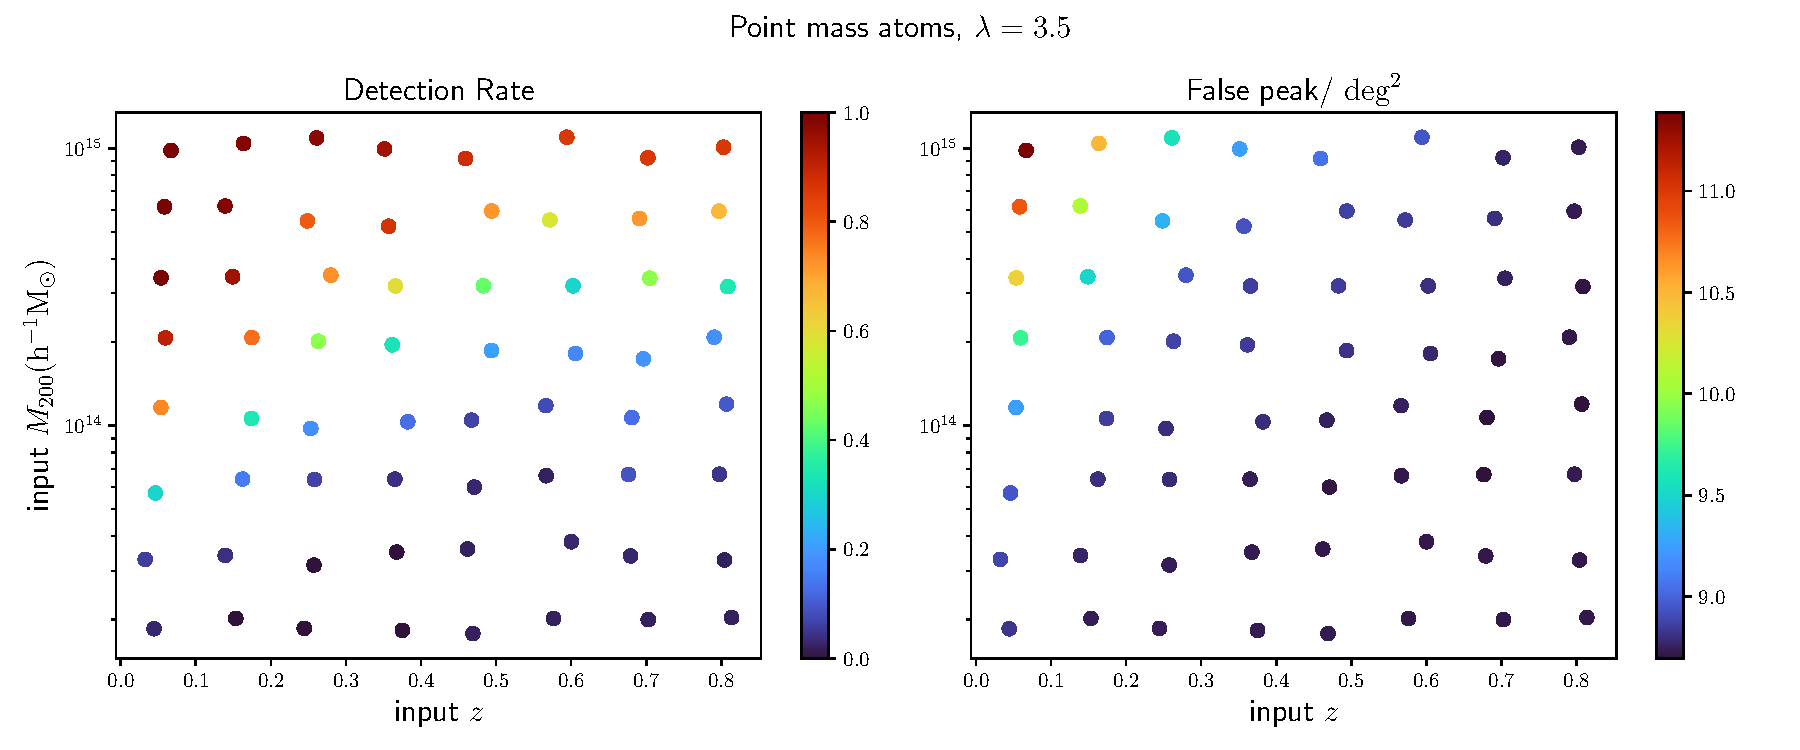
\includegraphics[width=1.0\textwidth]{detfalseRate_f1-1.pdf}
 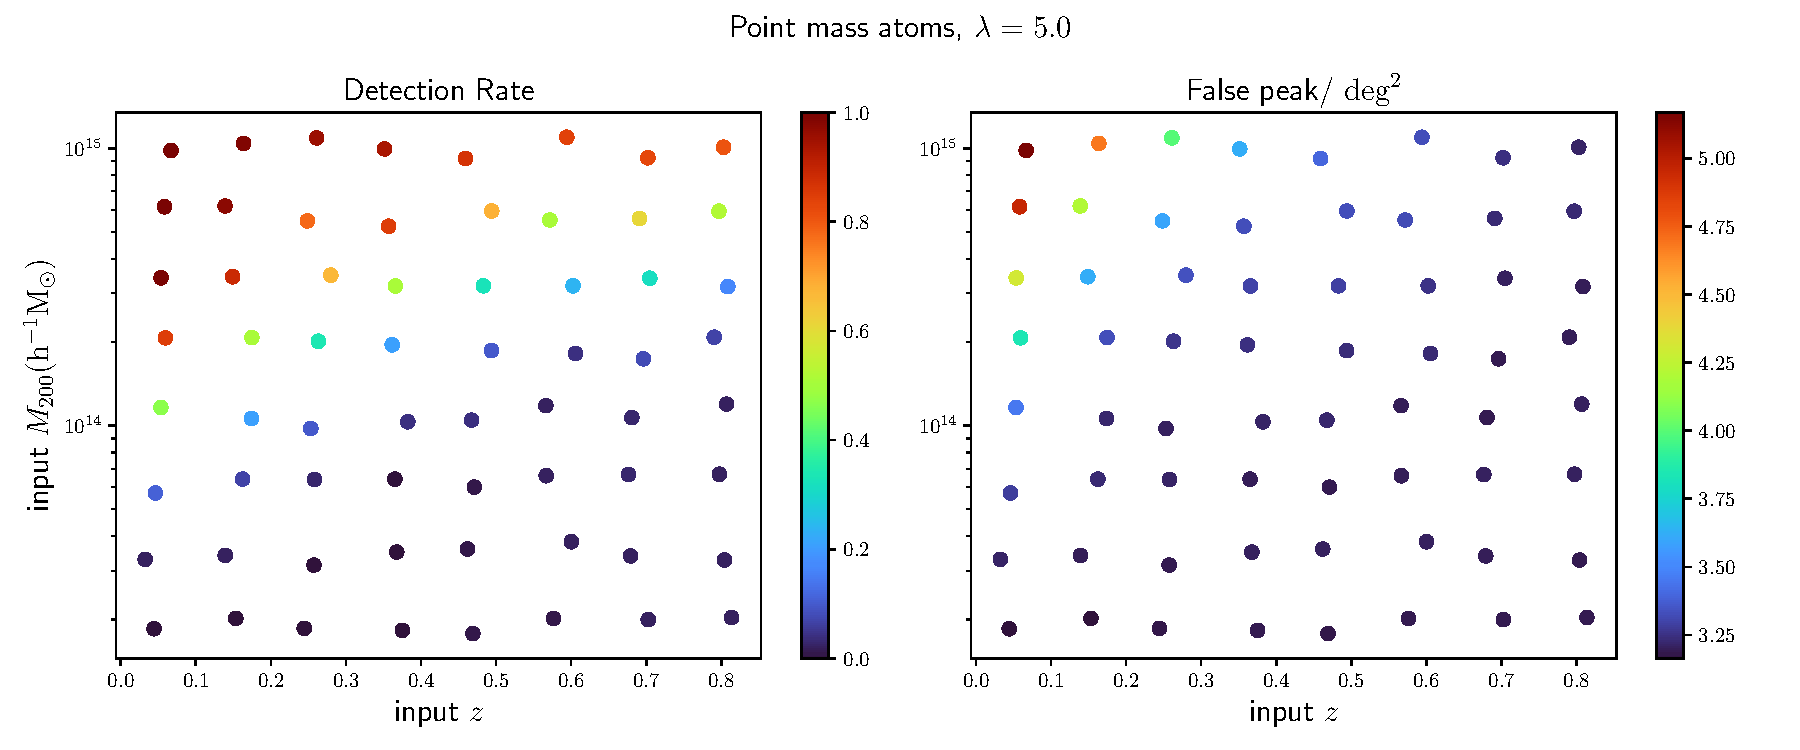
\includegraphics[width=1.0\textwidth]{detfalseRate_f1-3.pdf}
 \caption{The upper panels show the halo detection rate and the number of false
     peak per square degree for mass map reconstructed with the point mass
     dictionary. The penalization paramter is set to $\lambda=3.5$ for the
     upper panels.  The lower panels show the results for $\lambda=5.0$.
        }\label{fig_detFalsRatePM}
\end{figure*}

In this subsection, we test the performance of our algorithm with the default
setup that models the matter density field with multi-scale NFW atoms. The
dictionary is constructed with three frames of different NFW comoving scale
radius: $0.12~h^{-1}$ Mpc, $0.24~h^{-1}$ Mpc, and $0.36~h^{-1}$ Mpc.  The
truncation radius (concentration) is set to four times the scale radius for the
atoms in the dictionary.

We test the algorithm with different regularization parameters for the
preliminary lasso estimation which range from $3.5$ to $5.0$. The
regularization parameter for the adaptive lasso is set to
$\lambda_{\rm{als}}=\lambda_{\rm{ls}}^{\tau+1}$.
Here, we note that both the preliminary lasso estimation and the final adaptive
estimation select the modes with signal to noise ratios (SNRs) greater than
$\lambda_{\rm{ls}}$ in each iteration. While the final adaptive lasso
estimation further enhances the growth of the modes with preliminary
estimations greater than $\lambda_{\rm{ls}}$.

This paper does not go beyond the resolution limit defined by the Gaussian
smoothing kernel with the scale: $1.\arcmin 5$ and the pixel scale
that equals $1\arcmin$. We smooth the reconstructed density with the same
Gaussian kernel in each lens redshift plane.

We detect the peaks on the density map after the reconstruction. The stacked
$2$-D histogram, from all of the simulations, for the offsets of the detected
peak positions from the input halos' positions is shown in the left panel of
Figure \ref{fig_detoffsets}.

For each simulation, we find the positive peak closest to the input position
(in the pixel unit), and if the closest peak lay inside the region denoted with
the dashed box in the left panel of Figure \ref{fig_detoffsets}, we take it as
a true peak detection of the input halo. Other detected peaks, which include both
positive and negative peaks, are taken as false peaks. The right
panel of Figure \ref{fig_detoffsets} shows the average redshift of true
detections for each halo. The estimated redshifts are lower than the true
redshifts by about $0.03$ for halos in the low-redshift range ($z\leq 0.4$).
For halos at $0.4<z\leq 0.85$, the relative redshift bias is below $0.5\%$.

Figure \ref{fig_detFalsRateNFW} shows the detection rate (left panels) and the
number of false peaks per square degree (right panel) for each simulated halo.
The figure include results of different penalization parameters: $\lambda=3.5$
(upper panel) and $\lambda=5.0$ (lower panel).  We find that with the increase
of the penalization parameter, the detection rate decreases. On the other hand,
the number of false peaks also decreases.

Figure \ref{fig_peakHist} shows the histograms, which are normalized by the
number of simulations, for all detected peaks with different penalization
parameters. We also plot the corresponding histograms for peaks detected from
pure noise fields for comparison. From the left panels of Figure
\ref{fig_NFWvsPM}, which show the $3$-D density maps reconstructed with
different penalization parameters for a halo with $M_{200}=10^{15.02}
~h^{-1}M_{\odot}$ at redshift $0.164$ , we also find that the number of false
peaks significantly decreases as the penalization parameter increases.

\subsection{Point mass atoms}
\label{subsec:test-pm}

\begin{figure*}
 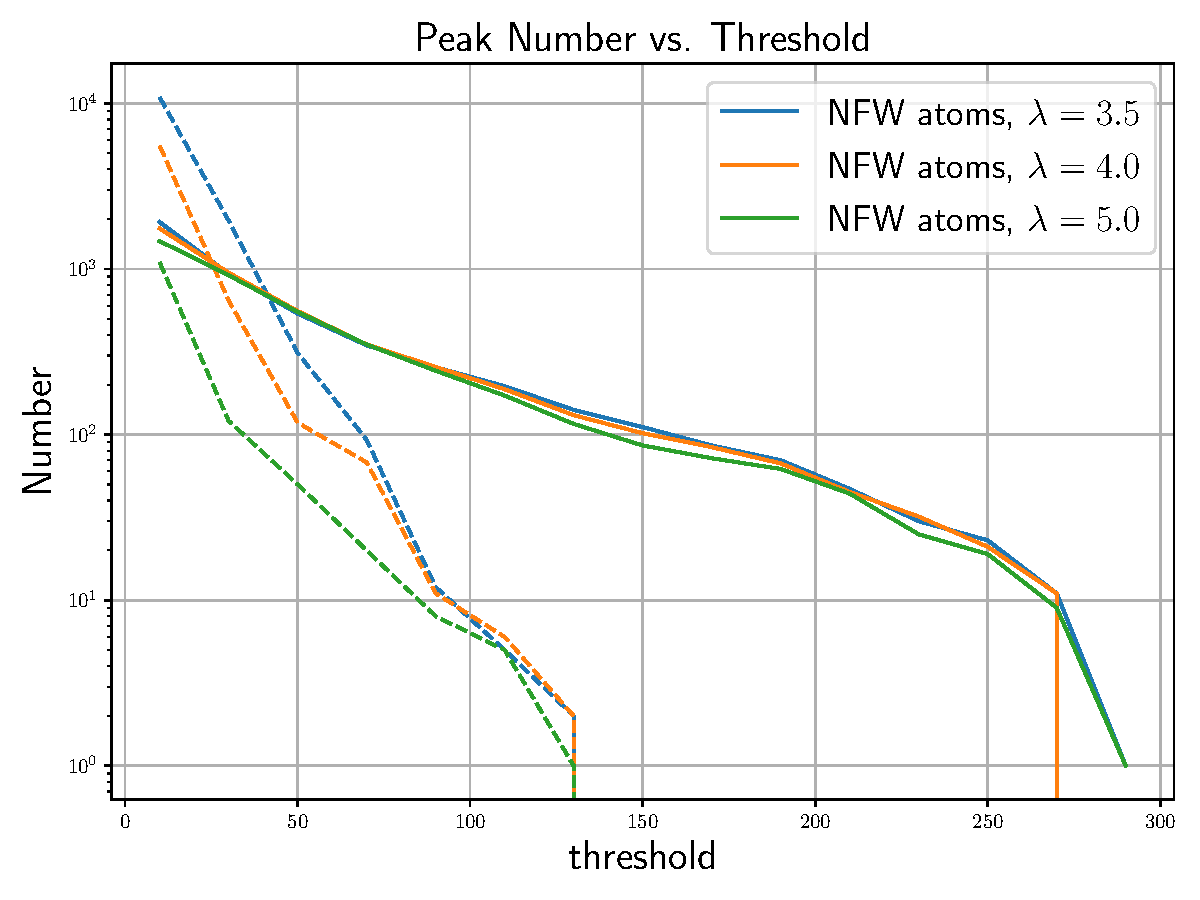
\includegraphics[width=1.0\textwidth]{detfalse_threshold.pdf}
 \caption{The left panel and the middle panel show the halo detection rates
     with different input masses and redshifts. The detections are performed on
     the mass maps reconstructed with $\lambda=5.0$, and the detection
     thresholds are set to $1.5\sigma$ and $3.0\sigma$ of the peak's standard
     deviation of the noise field, respectively. The right panel shows the
     numbers of false peaks per square degree as a function of selection
     thresholds. The corresponding false peaks per square degree for thresholds
     of $1.5\sigma$ and $3.0\sigma$ are about $0.022~\rm{deg}^{-2}$ and
     $0.004~\rm{deg}^{-2}$.
    }\label{fig_detfalse_threshold}
\end{figure*}

In this subsection, we show the results for the setup, which substitutes the
default NFW dictionary with the point mass dictionary, to compare with the
default setup.  The regularization parameter for the preliminary lasso is set
to $3.5$ and $5.0$.  Inspired by \citet{structureAdaLasso-Pramanik2020}, which
propose to incorporate external group information into different adaptive lasso
penalization weights by setting the penalization weights for projection
coefficients in the same group to the average of the adaptive weights in this
group, we smooth the preliminary lasso estimation in each lens redshift bin
with a top-hat filter of comoving scale $0.25~h^{-1}$ Mpc. The smoothed
preliminary lasso estimation is denoted as $\hat{x}^{\rm{ls}}_{\rm{sm}}$, and
the penalization weights are set to $1/\abs{\hat{x}^{\rm{ls}}_{\rm{sm}}}^\tau$.
The regularization parameter for the adaptive lasso is set to
$\lambda_{\rm{als}}=\lambda_{\rm{ls}}$.

As we have done on the NFW dictionary's reconstruction, we smooth the
reconstructed density maps with the Gaussian kernel (scale radius equals
$1.\arcmin 5$) in each lens redshift plane.

Figure \ref{fig_detFalsRatePM} shows the detection rate (left panels) and the
number of false peaks per square degree (right panel) for each setup of halo
mass and redshift.
This figure includes results of different penalization parameters:
$\lambda=3.5$ (upper panel) and $\lambda=5.0$ (lower panel). The right panels
of Figure \ref{fig_NFWvsPM} show the $3$-D density maps reconstructed with
different penalization parameters for a halo with $M_{200}=10^{15.02}
~h^{-1}M_{\odot}$ at redshift $0.164$.
Comparing with the results of the NFW dictionary, we find that the number of
false peaks in the mass map reconstructed with the point mass dictionary is
much larger than the NFW dictionary.

As demonstrated in the right panels of Figure \ref{fig_NFWvsPM}, the mass
reconstructions with the point mass dictionary tend to assign masses to
several different redshift bins in the neighboring region of the halo center.
While the NFW dictionary produces consistent mass reconstructions.
Since the NFW atoms' profiles are more consistent with the mass profiles of the
input halos than the profile of a point mass, there are less false structures
reconstructed with the NFW dictionary.

\section{Summary}
\label{sec:Sum}

We develop a novel method to reconstruct $3$-D density contrast maps from
weak-lensing shear measurements and photometric redshift estimations.  Our
method models $3$-D density contrast maps as summations of NFW atoms with
difference comoving radius.  With the prior assumption that the clumpy mass
sparsely distributes in the $3$-D space, the density field is reconstructed
using the adaptive lasso algorithm \citep{AdaLASSO-Zou2006}. The method is
tested with realistic simulations using HSC-like shape estimation error and
HSC-like photo-$z$ uncertainty.

We will apply the method to the shear measurements of the HSC survey
\citep{HSC1-catalog,FPFSHSC1-Li2020} to perform galaxy cluster detection in our
future work.  Here, we note that, when detecting galaxy clusters from the weak
lensing mass maps in real observations \citep{HSC1-massMap-cluster}, peaks
higher than an ad-hoc threshold is chosen as galaxy cluster candidates to
suppress the number of false detections. The threshold is set to a few times
the peak's standard deviation of the noise field (shear estimation error
field). We use different detection thresholds to detect peaks from the mass
maps reconstructed with $\lambda=5.0$. The left and middle panels of Figure
\ref{fig_detfalse_threshold} show the detection rates for halos with different
mass and redshift with detection thresholds set to $1.5\sigma$ and $3.0\sigma$
of the noise field, respectively. The right panel of Figure
\ref{fig_detfalse_threshold} shows the numbers of false detections as a
function of detection thresholds.

The findings of this paper are summarized as follows:
\begin{enumerate}
 \item The lasso algorithm's solution suffers from a smear of structure in
     the line of sight direction even in the absence of shape noise, and the
     adaptive lasso algorithm significantly removes the line of sight smear of
     structure.
 \item The algorithm is able to detect halo with minimal mass limits of
     $10^{14.0} M_{\odot}/h$, $10^{14.7} M_{\odot}/h$, $10^{15.0} M_{\odot}/h$
     for the low ($z<0.3$), median ($0.3\leq z< 0.6$) and high ($0.6\leq z<
     0.85$) redshifts, respectively, with a false detection of 0.022/deg$^2$.
 \item The estimated redshifts of the halos detected from the reconstructed mass
     maps are lower than the true redshift by about $0.03$ for halos at low
     redshifts ($z\leq 0.4$).  The relative redshift bias is below $0.5\%$ for
     halos at $0.4<z\leq 0.85$.
\end{enumerate}

\section*{Acknowledgements}
We thank Yin Li and Jiaxin Han for useful discussions.

This work was supported by Global Science Graduate Course (GSGC) program of
University of Tokyo and JSPS KAKENHI (JP19J22222).
\bibliographystyle{aasjournal}
\bibliography{citation}

\end{document}
